\pdfminorversion=4
\documentclass[compress,10pt]{beamer}
%For no animations, add handout to [] options
%For no figures or top banner, add draft to [] options
%apsectratio=169 (16:9) or 54 (5:4) or 43 (4:3) or 32 (3:2)

%Load the myriad packages
\usepackage{color}
\usepackage{amssymb,amsmath}
\usepackage{textcomp}
\usepackage{graphicx}
\usepackage{tikz}
%\usepackage[numbers, super]{natbib}
\usepackage{grffile} %spaces in file names
\usepackage{parskip}
%\usepackage[T1]{fontenc} %for sc and bf
%\usepackage{times}
\usepackage{wasysym}
\usepackage{bigstrut}
\usepackage{epstopdf}
%\usepackage[dvipsnames]{xcolor}
%\usepackage{enumitem}
%\setlist{nolistsep} % or \setlist{noitemsep} to leave space around whole list
% Load some optional sub-parts of PGF
%\usetikzlibrary{decorations.pathmorphing}
%\usetikzlibrary{positioning}
%\usetikzlibrary{calc}
%\usetikzlibrary{shapes.geometric}
%\usepackage{pgfplots}
%\usepackage{rotating}
%\usepackage[no-math]{fontspec}
%\usepackage{xltxtra}
%\usepackage{xunicode}
%\defaultfontfeatures{Mapping=tex-text}
%%\setsansfont[Mapping=tex-text]{Optima}
%\setsansfont[Mapping=tex-text]{Helvetica Neue}
% Optional for code samples
%
%singular
\newcommand{\fref}[1]{Fig.~\ref{fig:#1}}
\newcommand{\Fref}[1]{Figure~\ref{fig:#1}}
\newcommand{\eref}[1]{Eq.~(\ref{eq:#1})}
\newcommand{\Eref}[1]{Equation~(\ref{eq:#1})}
\newcommand{\tref}[1]{Table~\ref{tab:#1}}
%plural
\newcommand{\frefs}[2]{Figs.~\ref{fig:#1} and \ref{fig:#2}}
\newcommand{\Frefs}[2]{Figures~\ref{fig:#1} and \ref{fig:#2}}
\newcommand{\erefs}[2]{Eqs.~(\ref{eq:#1}) and (\ref{eq:#2})}
\newcommand{\Erefs}[2]{Equations~(\ref{eq:#1}) and (\ref{eq:#2})}
\newcommand{\trefs}[2]{Tables~\ref{tab:#1} and \ref{tab:#2}}
%range
\newcommand{\frefss}[2]{Figs.~\ref{fig:#1} - \ref{fig:#2}}
\newcommand{\Frefss}[2]{Figures~\ref{fig:#1} - \ref{fig:#2}}
\newcommand{\erefss}[2]{Eqs.~(\ref{eq:#1}) - (\ref{eq:#2})}
\newcommand{\Erefss}[2]{Equations~(\ref{eq:#1}) - (\ref{eq:#2})}
\newcommand{\trefss}[2]{Tables~\ref{tab:#1} - \ref{tab:#2}}
%misc.
\newcommand{\nn}[1]{\ensuremath{^{#1}}} %[1] is # of commands
\newcommand{\keff}{\ensuremath{{k_\mathrm{eff}}}}
\newcommand{\kinf}{\ensuremath{{k_\infty}}}
\newcommand{\alphaT}{\ensuremath{{\alpha_{_T}}}}
\newcommand{\SN}{\ensuremath{{\text{S}_\text{N}}}}
\newcommand{\order}[1]{\ensuremath{\mathcal{O}\left(#1\right)}}
%Note: tarticle has ``several'' changes from article
%in this vein.
% some simplifying commands
\newcommand{\eg}{{\it e.g.}}
\newcommand{\ie}{{\it i.e.}}
\newcommand{\etal}{{\it et al.}}
\newcommand{\acite}[1]{{\bf(Add Citation: #1)}}
\newcommand{\E}{\mathcal{E}}
% derivative - d
\newcommand{\ud}{\,\mathrm{d}}
% bold unit vector n-hat
\newcommand{\nhat}{\hat{\bf n}}
\newcommand{\tensor}[1]{\mathcal{#1}}
\renewcommand{\vec}[1]{\mathbf{#1}}
\newcommand{\om}{\boldsymbol{\Omega}}
%

%Don't number backup slides
\newcommand{\backupbegin}{
    \newcounter{finalframe}
    \setcounter{finalframe}{\value{framenumber}}
}
\newcommand{\backupend}{
    \setcounter{framenumber}{\value{finalframe}}
}

%Colors!
\definecolor{maroon}{rgb}{0.5,0,0}
\definecolor{darkgreen}{rgb}{0,0.5,0}
\definecolor{amber}{rgb}{1.0, 0.49, 0.0}

\newcommand{\tcr}[1]{\textcolor{red}{#1}}
\newcommand{\tcb}[1]{\textcolor{blue}{#1}}
\newcommand{\tcm}[1]{\textcolor{magenta}{#1}}

%Get rid of navigation icons
\setbeamertemplate{navigation symbols}{}
\useoutertheme{infolines}

\setbeamercovered{transparent}
\usepackage{lipsum}

%Aggie-themed
\pgfdeclareimage[height=0.1in]{TAMUlogo}{images/tamu_engineering.png}
\pgfdeclareimage[height=0.45in]{CERTlogo}{images/CERT_logo.png}
\logo{\raisebox{-8pt}{\pgfuseimage{TAMUlogo} \hspace{1pt} \pgfuseimage{CERTlogo}}}
\titlegraphic{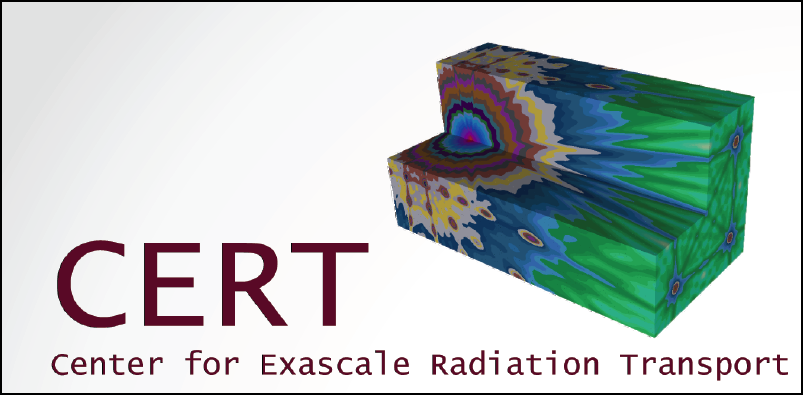
\includegraphics[height=0.20\textheight]{images/CERT_logo.png}}

%%%%%%%%%%%%%%%%%%%%%%%%%%%%%%%%%%%%%%%%%%%%%%%%%%%%%%%%%%%%%%%
% Optional packages, used to show off certain tricks

\newlength \figwidth
\setlength \figwidth {0.5\textwidth}

\setlength{\leftmargin}{-2cm}
\setlength{\rightmargin}{-2cm}

%%%%%%%%%%%%%%%%%%%%%%%%%%%%%%%%%%%%%%%%%%%%%%%%%%%%%%%%%%%%%%%

\mode<presentation>
{
    \usepackage[english]{babel}
    \usetheme{Frankfurt}

    %Make it Aggie Maroon
    \usecolortheme[RGB={80,0,0}]{structure}

    % This will typeset only the frames (or slides) that have the given label ("current" in this case).
    %  \includeonlyframes{current}
}

\title[DSA using DFEM for Massively Parallel Transport]{Diffusion Synthetic Acceleration for Massively-Parallel Transport Sweeps using a Discontinuous Finite element Method}

\author[Ragusa]{\Large Jean C. Ragusa, Michael W. Hackemack} 

%TAMU
\institute[Texas A\&M University]{\scriptsize Department of Nuclear Engineering\\
Texas A\&M University \\
College Station, TX, USA 77843\\[1ex]
\href{mailto:jean.ragusa@tamu.edu}{jean.ragusa@tamu.edu}}

\date[December 3, 2015]

% You can override the default acknowledgment, and address if you want
%\acknowledgement{*Submitted in partial fulfillment of the requirements of NUEN 610 \\
%(Nuclear Reactor Design)}
%\address{Nuclear Engineering Department \\
%            Texas A\&M University \\
%            College Station, TX 77843-3133}}

% If you don't want the menu section outline above the title, do this:
%\setbeamertemplate{headline}{}

\renewcommand{\ss}{ss}
\vfuzz=2pt

%%%%%%%%%%%%%%%%%%%%%%%%%%%%%%%%%%%%%%%%%%%%%%%%%%%%%%%%%%%%%%%%%%%%%%%%%%%%%%%%%%%%%%%%%%%%%
\begin{document}

%%%%%%%%%%%%%%%%%%%%%%%%%%%%%%%%%%%%%%%%%%%%%%%%%%%%%%%%%%%%%%%%%%%%%%%%%%%%%%%%%%%%%%%%%%%%%
%  All this typeout stuff simply gets printed to the screen as the document
% is compiled.  It helps get stuff working
\typeout{***********************************************************************************}
\typeout{titlepage}

\begin{frame}[label=title,plain]
    \titlepage
\end{frame}

%%%%%%%%%%%%%%%%%%%%%%%%%%%%%%%%%%%%%%%%%%%%%%%%%%%%%%%%%%%%%%%%%%%%%%%%%%%%%%%%%%%%%%%%%%%%%%
\typeout{***********************************************************************************}
\typeout{TOC}

\begin{frame}[shrink,label=toc,plain]%[plain]
    \frametitle{Outline}
    \vspace{1.1cm}
    \tableofcontents
\end{frame}

%%%%%%%%%%%%%%%%%%%%%%%%%%%%%%%%%%%%%%%%%%%%%%%%%%%%%%%%%%%%%%%%%%%%%%%%%%%%%%%%%%%%%%%%%%%%%%
%
\section{Motivation for this Work}
%%%%%%%%%%%%%%%%%%%%%%%%%%%%%%%%%%%%%%%%%%%%%%%%%%%%%%%%%%%%%%%%%%%%%%%%%%%%%%%%%%%%%%%%%%%%%
\typeout{***********************************************************************************}
\typeout{Motivation}
%---------------------------
\begin{frame}[t]\frametitle{Motivation}
\vspace{-2mm}
\begin{block}{Parallel Transport Sweeps}
{\small
\begin{itemize}
\item Massively-parallel transport sweeps is a mature technology 
\item PDT's weak scaling demonstrated up to \tcr{1.5 million cores} for \tcb{logically-block grids}
(and ongoing work for parallel transport sweeps on \tcb{unstructured grids})
\item Enabling technologies:
\begin{enumerate}
\item \tcb{Discrete ordinates} angular discretization (decouples directions in the streaming+collision transport operator)
\item Discontinuous Finite Element Method (\tcb{DFEM}) for spatial discretization (``invert the transport operator in a given direction on a cell-by-cell basis'')
%\begin{itemize}
%\item Out of the family of DFEM basis functions, PWLD is particularly useful to deal with parallel unstructured meshing
%\end{itemize}
\item \tcb{Aggregation} of spatial cells and angular directions (and energy groups) into work-unit '`tasks'' and \tcb{task scheduling}  
\end{enumerate}
\end{itemize}
}
\end{block}
\vspace{-1mm}
\begin{block}{Typical Drawbacks of Transport Sweeps}
{\small
Slow iterative convergence in optically thick configurations, $\left( \sigma_{t,g} \cdot \text{diam} (\mathcal{D}) \right) \gg 1$
\begin{enumerate}
\item \tcr{within an energy group}: 
$\sigma_s^{g \rightarrow g} / {\sigma_{t,g}} \approx  1$ 
\item \tcr{thermal upscattering} when solved using a Gauss-Seidel approach for material with little thermal absorption
\end{enumerate}
}
\end{block}

\end{frame}
%%%%%%%%%%%%%%%%%%%%%%%%%%%%%%%%%%%%%%%%%%%%%%%%%%%%%%%%%%%%%%%%%%%%%%%%%%%%%%%%%%%%%%%%%%%%%%

%%%%%%%%%%%%%%%%%%%%%%%%%%%%%%%%%%%%%%%%%%%%%%%%%%%%%%%%%%%%%%%%%%%%%%%%%%%%%%%%%%%%%%%%%%%%%
\typeout{***********************************************************************************}
\typeout{The DGFEM $S_N$ Transport Equation}
\begin{frame}[t]\frametitle{Iterative Procedure}

\begin{block}{Source Iteration} {\small
\begin{equation*}
\begin{aligned}
 \psi^{(\ell+1)} &= {\bf L}^{-1} \left( {\bf M} {\bf \Sigma} \phi^{(\ell)}  +  {\bf Q} \right) \\
\phi^{(\ell+1)} &= {\bf D}  \psi^{(\ell+1)}
\end{aligned}
\end{equation*}
The operation ${\bf L}^{-1}$ is a transport sweep.\\
}
\end{block}

\begin{block}{Operator Terms} {\small
\begin{tabular}{ll}
${\bf L}$ - streaming + collision operator & ${\bf L } = diag(L_1, \ldots, L_{n_\Omega})$ \\
${\bf M}$ - moment-to-discrete operator &
${\bf D}$ - discrete-to-moment operator \\
${\bf \Sigma}$ - scattering operator &
${\bf Q}$ - source operator \\
\end{tabular}
}
\end{block}

\begin{block}{GMRES equivalent form} {\small
Sweep-Preconditioning
\[
{\bf  ( I - DL^{-1} M\Sigma) \Phi = D L^{-1} Q}
\]
}
\end{block}
\end{frame}
%%%%%%%%%%%%%%%%%%%%%%%%%%%%%%%%%%%%%%%%%%%%%%%%%%%%%%%%%%%%%%%%%%%%%%%%%%%%%%%%%%%%%%%%%%%%%
\typeout{***********************************************************************************}
\typeout{The DGFEM $S_N$ Transport Equation}
\setbeamerfont{frametitle}{size=\small}
\begin{frame}[t]\frametitle{Synthetic Acceleration}

\begin{block}{Transport sweep and iteration error}{\small
\begin{columns}

\column{0.60\textwidth}
\begin{equation*}
\begin{aligned}
{\bf L} \psi              &= {\bf M\Sigma} \phi          +{\bf Q} \\
{\bf L} \psi^{(\ell+1/2)} &= {\bf M\Sigma} \phi^{(\ell)} +{\bf Q} + {\bf M\Sigma} (\phi^{(\ell+1/2)}-\phi^{(\ell+1/2)})\\
\noindent\rule{1.5cm}{0.4pt} &\noindent\rule{5.8cm}{0.4pt} \\
{\bf L} \delta \psi^{(\ell+1/2)} &- {\bf M\Sigma} \delta \phi^{(\ell+1/2)} = {\bf M\Sigma} (\phi^{(\ell+1/2)}-\phi^{(\ell)}) = {\bf R}^{(\ell+1/2)}
\end{aligned}
\end{equation*}

\column{0.40\textwidth}
\begin{equation*}
\begin{aligned}
\delta \psi^{(\ell+1/2)} &\equiv \psi - \psi^{(\ell+1/2)} \\
\delta \phi^{(\ell+1/2)} &\equiv {\bf D} \delta \psi^{(\ell+1/2)}
\end{aligned}
\end{equation*}
\end{columns}
}
\end{block}

\begin{block}{Error approximation and update}{\small
If we could exactly solve for the error, then the solution could be obtained immediately:
\begin{equation*}
\phi^{(\ell+1)} = \phi^{(\ell+1/2)} + \delta \phi^{(\ell+1/2)}
\end{equation*}
However, this is just as difficult as the original transport problem. Instead, we estimate the error using low-order operators:
\begin{equation*}
{\bf A} \delta \phi^{(\ell+1/2)} = \tilde{{\bf R}}^{(\ell+1/2)}
\end{equation*}
${\bf A}$ is a low-order diffusion operator.
}
\end{block}

\end{frame}
%%%%%%%%%%%%%%%%%%%%%%%%%%%%%%%%%%%%%%%%%%%%%%%%%%%%%%%%%%%%%%%%%%%%%%%%%%%%%%%%%%%%%%%%%%%%%%
%
\section[DSA on Polytopes]{Diffusion Synthetic Acceleration on Polytopes using a DFEM technique}
\subsection{Brief review of DSA Theory}
%%%%%%%%%%%%%%%%%%%%%%%%%%%%%%%%%%%%%%%%%%%%%%%%%%%%%%%%%%%%%%%%%%%%%%%%%%%%%%%%%%%%%%%%%%%%%
\typeout{***********************************************************************************}
\typeout{DSA}
%---------------------------
\begin{frame}[t]\frametitle{Diffusion Synthetic Acceleration}

\begin{block}{Desirable properties for the diffusion operator ${\bf A}$ } {\small 
	\begin{itemize}
		\item Symmetric Positive-Definite (SPD) in order to use efficient solvers (e.g., CG)
		\item Availability of suitable preconditioners (e.g., PCG with Algebraic MultiGrid)
		\item Can handle concave and degenerate polygonal/polyhedral cells
		\item Discontinuous FEM (same DFEM space as transport to avoid the need for a discontinuous update when using CFEM for diffusion)
	\end{itemize} }
\end{block}

\begin{block}{} {\small 
     		\begin{align*}
 	 		{ \small -{\bf \nabla} \cdot D {\bf \nabla} \Phi ({\bf r}) + \sigma \Phi ({\bf r}) = q ({\bf r}), \qquad  {\bf r} \in \mathcal{D} }
        	\end{align*} 
General Boundary Conditions:
		\begin{align*}
 	 		{ \small \Phi ({\bf r})  = \Phi_0 ({\bf r}) , \qquad {\bf r} \in \partial \mathcal{D}^d } \\
 	 		{ \small -D \partial_n \Phi ({\bf r})  = J_0 ({\bf r}) , \qquad {\bf r} \in \partial \mathcal{D}^n } \\
 	 		{ \small \frac{1}{4} \Phi ({\bf r})  + \frac{1}{2}D \partial_n \Phi ({\bf r})  = J^{inc} ({\bf r}) ,  \qquad {\bf r} \in \partial \mathcal{D}^r}
        		\end{align*} } \vspace{-0.25cm}
\end{block}

\end{frame}

\subsection{Symmetric Interior Penalty (SIP) Form for Diffusion}
%%%%%%%%%%%%%%%%%%%%%%%%%%%%%%%%%%%%%%%%%%%%%%%%%%%%%%%%%%%%%%%%%%%%%%%%%%%%%%%%%%%%%%%%%%%%%
\typeout{***********************************************************************************}
\typeout{DSA}
%---------------------------
\begin{frame}[t]\frametitle{Symmetric Interior Penalty (SIP) Form for Diffusion}


\[
\text{Weak form: } \qquad a(\Phi,b) = \ell(b)
\]

\begin{block}{Bilinear Form}{\small
		\begin{gather*}
			 a( \Phi, b)  = \Big<  D \vec{\nabla}  \Phi , \vec{\nabla} b  \Big>_{\mathcal{D}} + \Big<  \sigma   \Phi ,  b  \Big>_{\mathcal{D}}    \\
			+  \Big\{ \kappa_e^{SIP} [\![   \Phi ]\!] , [\![  b ]\!]\Big\}_{E_h^i} - \Big\{  [\![   \Phi ]\!] , \{\!\{  D \partial_n b \}\!\}\Big\}_{E_h^i} -\Big\{ \{\!\{  D \partial_n  \Phi \}\!\} , [\![ b ]\!]\Big\}_{E_h^i} \\
			+ \Big\{ \kappa_e^{SIP}   \Phi ,   b \Big\}_{\partial \mathcal{D}^d} - \Big\{   \Phi  ,  D \partial_n b \Big\}_{\partial \mathcal{D}^d} - \Big\{   D 				\partial_n  \Phi ,   b \Big\}_{\partial \mathcal{D}^d}  +  \frac{1}{2} \Big\{    \Phi ,   b \Big\}_{\partial \mathcal{D}^r}
        	\end{gather*} }
\end{block}

\begin{block}{Linear Form}{\small
		\begin{align*}
			\ell (b) = \Big<  q, b  \Big>_{\mathcal{D}}  - \Big\{   J_{0}, b  \Big\}_{\partial \mathcal{D}^n} +  2 \Big\{   J_{inc}, b  \Big\}_{\partial 				\mathcal{D}^r} \\ + \Big\{ \kappa_e^{SIP}   \Phi_0 ,   b \Big\}_{\partial \mathcal{D}^d} - \Big\{   \Phi_0  ,  D \partial_n b \Big\}_{\partial 					\mathcal{D}^d} 
        	\end{align*} }
    \end{block}
\end{frame}
%---------------------------
\begin{frame}[t]\frametitle{SIP Penalty Coefficient}
\begin{block}{}{
	\begin{equation*}
		\kappa_e^{SIP} \equiv 
		\begin{cases}
		\frac{C_B}{2} \left(  \frac{D^+}{h^+} + \frac{D^-}{h^-}  \right) & , e \in E_h^i \\
		C_B \frac{D^-}{h^-}  & , e \in \partial \mathcal{D}
		\end{cases}
	\end{equation*}}
	\begin{equation*}
		C_B = c p (p+1)
	\end{equation*}
\end{block}
\begin{block}{}
$c$ - user defined constant ($c \geq 1$) \\
$p$ - polynomial order of the finite element basis ($1,2,3,...$) \\
$D^{(+/-)}$ - diffusion coefficient defined on the positive/negative side of a face\\
$h^{(+/-)}$ - orthogonal projection defined on the positive/negative side of a face
\end{block}
\begin{block}{}
\[
[\![ u ]\!] := u^+ - u^- \qquad  \{\!\{  u \}\!\} := \frac{u^+ + u^i}{2}
\]
	\begin{equation*}
		u^{\pm} = \lim_{s \rightarrow 0^{\pm}} u ({\bf r} + s {\bf n})
	\end{equation*}
\end{block}
\end{frame}
%---------------------------
\subsection{Modified Interior Penalty (MIP) form for DSA}
\begin{frame}[t]\frametitle{Modified Interior Penalty (MIP) Form}

Recall the DSA equation:
\begin{equation*}
{\bf A} \tcr{\delta \phi}^{(\ell+1/2)} = \tilde{{\bf R}}^{(\ell+1/2)}
\end{equation*}
 
\begin{block}{DSA Form}{\footnotesize
\begin{gather*}
\Big<  D \vec{\nabla} \tcr{\delta \Phi} , \vec{\nabla} b  \Big>_{\mathcal{D}} 
+ \Big<  \sigma \tcr{\delta  \Phi} ,  b  \Big>_{\mathcal{D}}    \\
+ \Big\{ \kappa_e^{MIP} [\![ \tcr{\delta  \Phi} ]\!] , [\![  b ]\!]\Big\}_{E_h^i} 
- \Big\{  [\![  \tcr{\delta \Phi} ]\!] , \{\!\{  D \partial_n b \}\!\}\Big\}_{E_h^i} 
- \Big\{ \{\!\{  D \partial_n \tcr{\delta \Phi} \}\!\} , [\![ b ]\!]\Big\}_{E_h^i} \\
+ \frac{1}{2} \Big\{  \tcr{\delta  \Phi} ,   b \Big\}_{\partial \mathcal{D}^{vac}} 
 = \Big<  R , b  \Big>_{\mathcal{D}}  -  \Big\{  \tcr{\delta J_{inc}}, b  \Big\}_{\partial \mathcal{D}^{ref}}
\end{gather*} 
}
\end{block}

\begin{block}{MIP Penalty Term}{\footnotesize
		\begin{align*}
			\kappa_e^{MIP} = \max\left(\frac{1}{4},  \kappa_e^{SIP}\right)
		\end{align*} }
	\end{block}
\end{frame}
%
%%%%%%%%%%%%%%%%%%%%%%%%%%%%%%%%%%%%%%%%%%%%%%%%%%%%%%%%%%%%%%%%%%%%%%%%%%%%%%%%%%%%%%%%%%%%%
\subsection{3D Fourier analysis results}
%---------------------------
\begin{frame}[t]\frametitle{3D DFEM DSA Analysis}
\centering
\vspace{0.2cm}
\includegraphics[width=0.32\textwidth]{images/3D_cart_mesh.eps} 
\includegraphics[width=0.32\textwidth]{images/3D_tri_mesh.eps}
\includegraphics[width=0.32\textwidth]{images/3D_rand_poly_mesh.eps}  \\
\vspace{0.2cm}
\includegraphics[width=0.32\textwidth]{images/3D_shes_poly_mesh.eps} 
\includegraphics[width=0.32\textwidth]{images/3D_sine_poly_mesh.eps} 
\includegraphics[width=0.32\textwidth]{images/3D_z_poly_mesh.eps} 
\end{frame}
%---------------------------

\subsection{}
\begin{frame}[t]\frametitle{Fourier analysis - 3D PWL basis functions}
\begin{columns}
\column{0.48\textwidth}
\begin{block}{$c=1$}
\centering
{}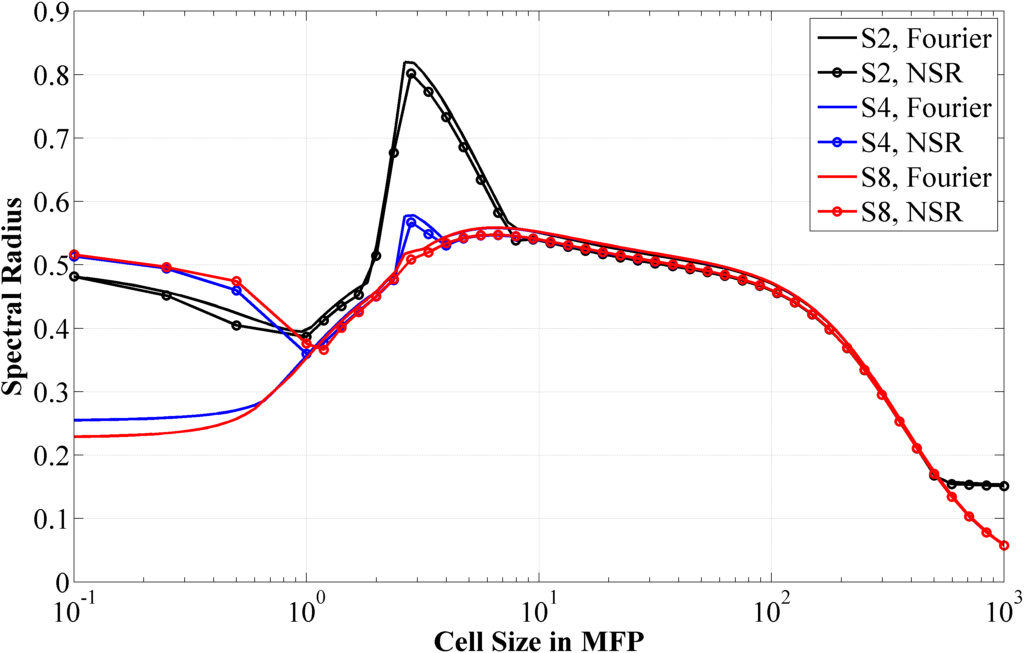
\includegraphics[width=0.8\textwidth]{images/SI_MIP_hex_C=1_LS2,4,8_F&NSR_PDT.png} \\
{}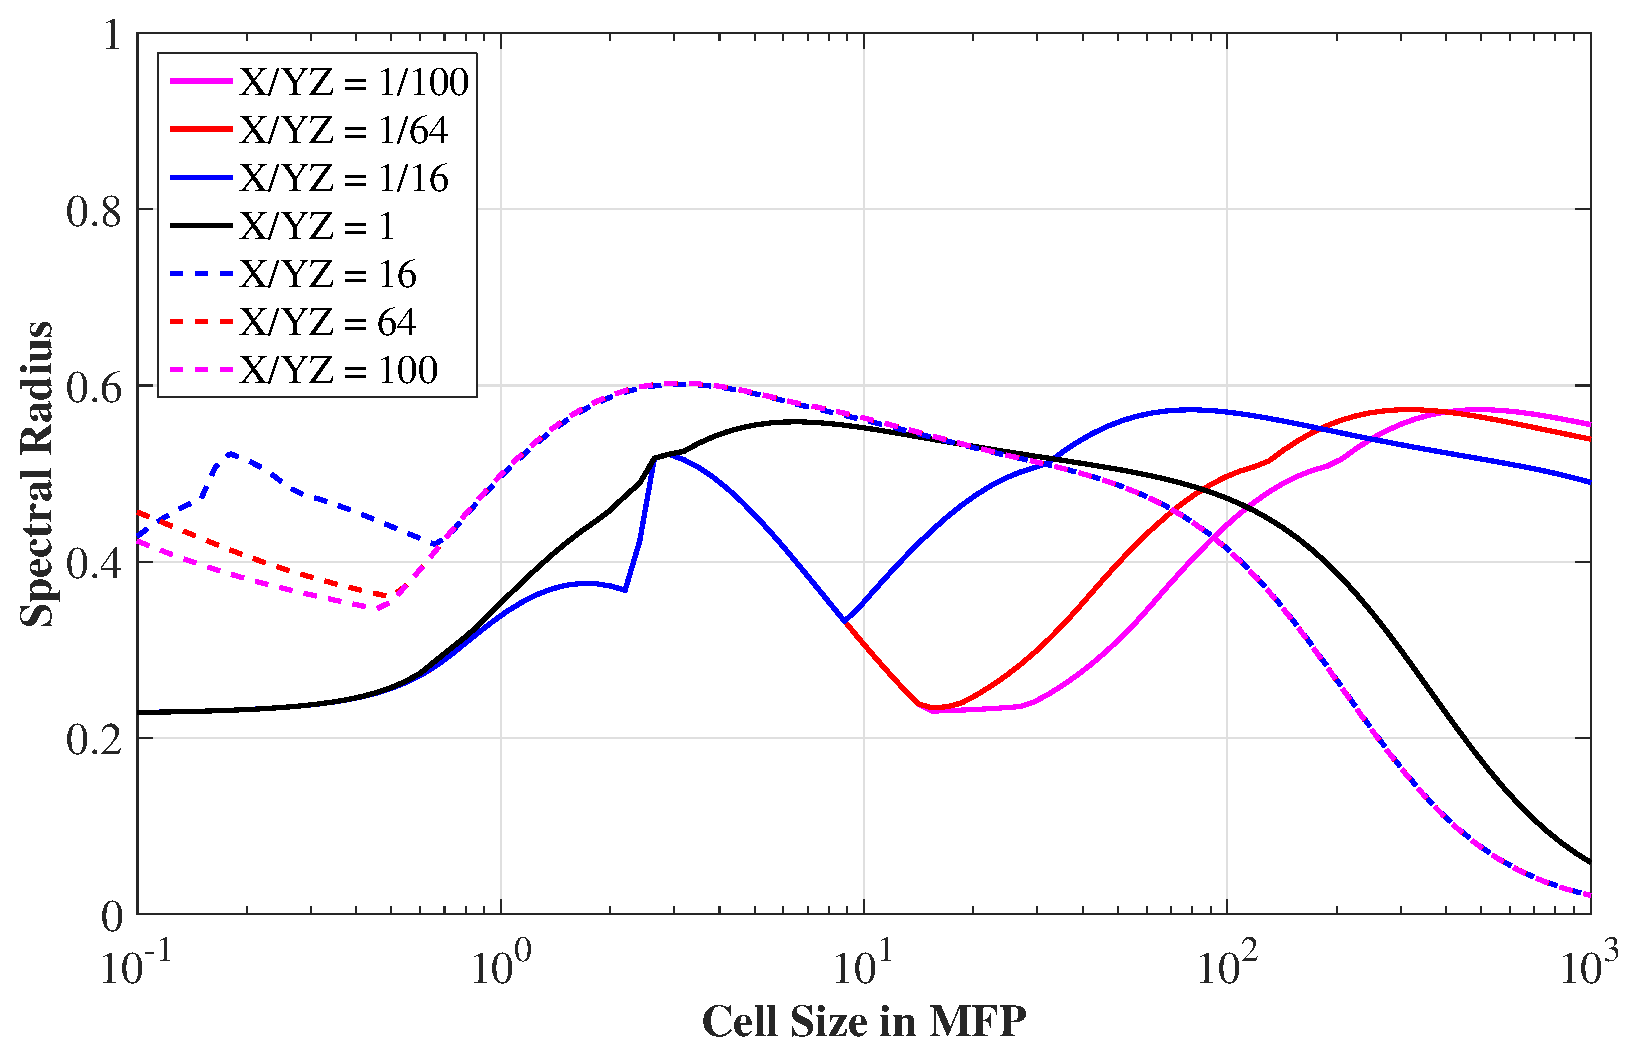
\includegraphics[width=0.8\textwidth]{images/SI_MIP_hex_LS8_C=1_AR.eps}
\end{block}
\column{0.48\textwidth}
\begin{block}{$c=4$}
\centering
{}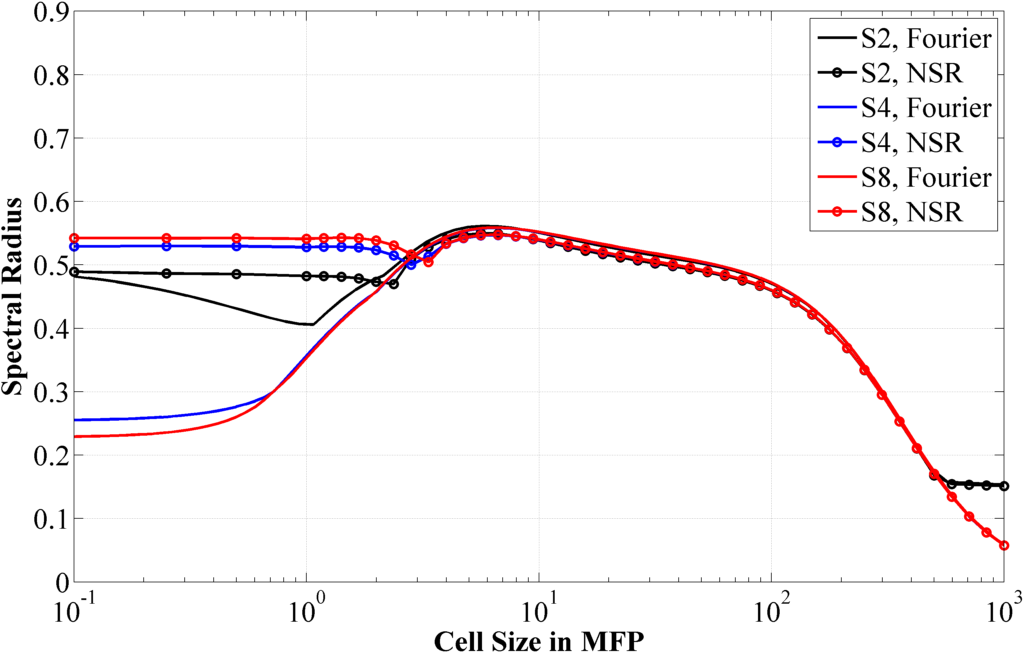
\includegraphics[width=0.8\textwidth]{images/SI_MIP_hex_C=4_LS2,4,8_F&NSR_PDT.png} \\
{}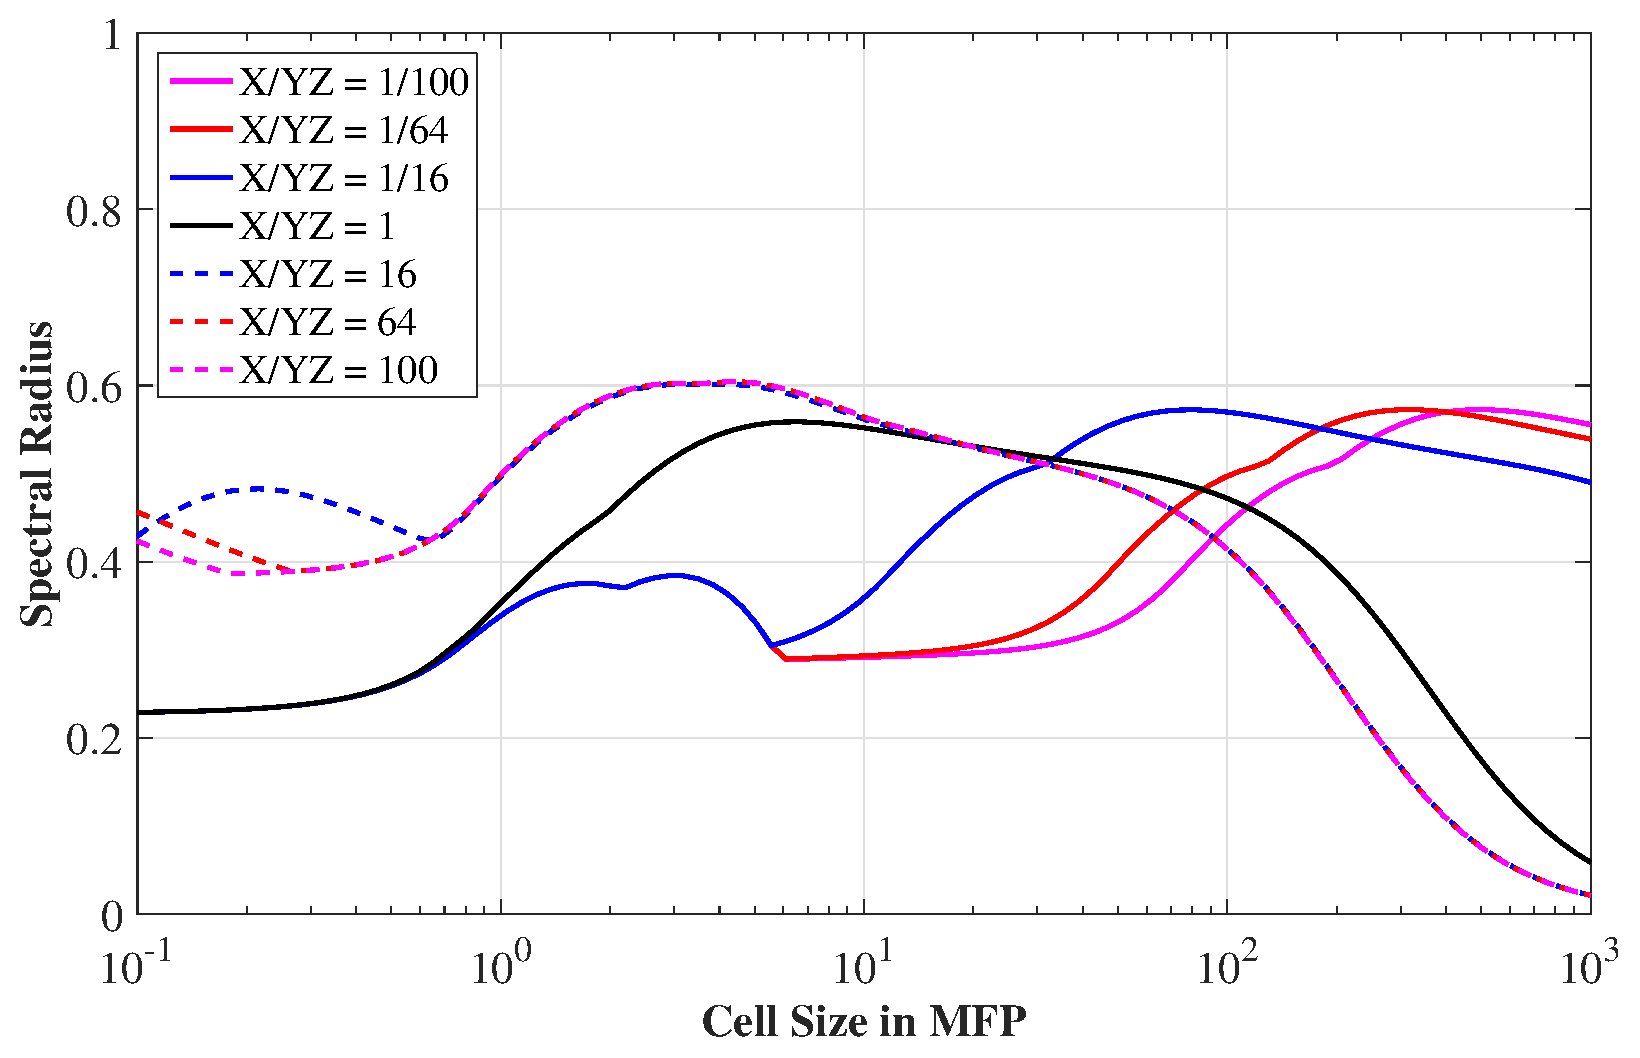
\includegraphics[width=0.8\textwidth]{images/SI_MIP_hex_LS8_C=4_AR.eps}
\end{block}
\end{columns}
\end{frame}
%---------------------------
\subsection{MIP-DSA results with PDT}

\begin{frame}[t]\frametitle{MIP DSA Timing Data with PDT on Vulcan using \tcr{HYPRE}}
\begin{figure}[t]
\centering
{}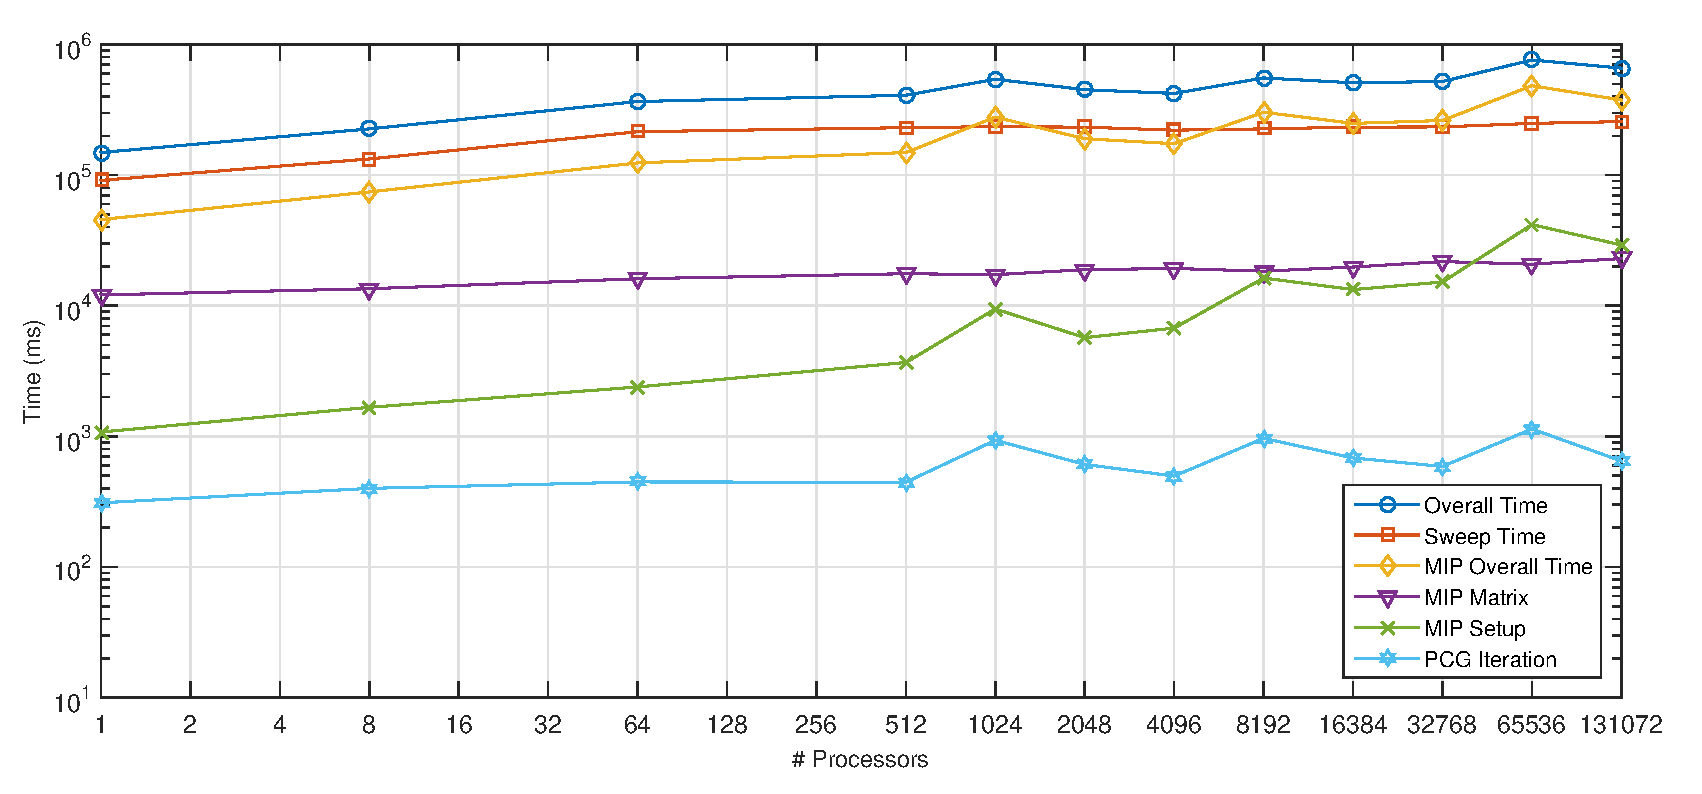
\includegraphics[width=0.75\textwidth]{images/Vulcan_DSA_Timing.eps}
\begin{block}{Problem Description}
	\begin{itemize}
	\item Modified Zerr problem - used optimal sweep aggregation parameters
	\begin{itemize}
	\item homogeneous cube - about 500 mfp and c=0.9999
	\item $S_8$ level-symmetric quadrature (80 directions total)
	\end{itemize}
	\item pointwise convergence tolerance of 1e-8
	\item SI precondition with MIP DSA using \tcr{HYPRE PCG and AMG} ($\sim$22 SI @ high core counts, and $\sim$10 CG iters/DSA)
	\end{itemize}
\end{block}
\end{figure}
\end{frame}


%---------------------------
\section{Acceleration of thermal upscattering iterations}
\subsection{Two-grid Acceleration of thermal upscattering}

\begin{frame}[t]\frametitle{Two-Grid Acceleration - Ideal for graphite and heavy-water configurations}
{\small
\vspace{-4mm}
\begin{columns}
\column{0.63\textwidth}
\begin{block}{Multigroup system of equations}{\footnotesize
Gauss-Seidel iterations over thermal groups:
\begin{equation*}
%\begin{aligned}
%{\bf L_{gg}} \psi_g &=  {\bf M} \sum_{g'=0}^G {\bf \Sigma}_{g g'} \phi_{g'} + {\bf Q}_g \\ 
{\bf L_{gg}} \psi_g^{(k+1/2)} = {\bf M} \sum_{g'=0}^g {\bf \Sigma}_{g g'} \phi_{g'}^{(k+1/2)} + {\bf M} \sum_{g'=g+1}^G {\bf \Sigma}_{g g'} \phi_{g'}^{(k)} + {\bf Q}_g
%\end{aligned}
\end{equation*}
}\end{block}
\begin{block}{Error and residual}{\footnotesize
\begin{equation*}
\begin{aligned}
{\bf L_{gg}} \delta \Psi_g^{(k+1/2)} &= {\bf M} \sum_{g'=0}^g {\bf \Sigma}_{g g'} \delta \Phi_{g'}^{(k+1/2)} + {\bf R}_g^{(k+1/2)} \\
{\bf R}_g^{(k+1/2)} &= {\bf M} \sum_{g'=g+1}^G {\bf \Sigma}_{g g'} \left(  \Phi_{g'}^{(k+1/2)} - \Phi_{g'}^{(k)}  \right)
\end{aligned}
\end{equation*}
}\end{block}
\vspace{-2mm}
\begin{block}{Solution update}{\footnotesize
\begin{equation*}
\begin{aligned}
&\delta \Phi_{g}^{(k+1/2)} = \tcb{\epsilon^{(k+1/2)}} \, \tcr{\xi_g}, \qquad \sum\displaylimits_{g=0}^{G} \tcr{\xi_g} = 1 \\
& \left({\bf \Sigma_t} - tril({\bf \Sigma_s})^{-1} \right) triu({\bf \Sigma_s}){\bf \tcr{\xi}} = \rho {\bf \tcr{\xi}}
\end{aligned}
\end{equation*}
}\end{block}

\column{0.35\textwidth}
\begin{block}{1G Error Diffusion System}{\footnotesize
\begin{equation*}
\vec{\nabla} \cdot \Big< D \Big> \vec{\nabla} \tcb{\epsilon} + \Big< \sigma \Big> \tcb{\epsilon} = \Big< R \Big>
\end{equation*} \\ \vspace{2mm}
\begin{equation*}
\begin{aligned}
&\Big< D \Big> = \sum\displaylimits_{g=0}^{G} D_g \tcr{\xi_g} \\
&\Big< \sigma \Big> = \sum\displaylimits_{g=0}^{G} \left(  \sigma_{t,g} \tcr{\xi_g} - \sum\displaylimits_{g'=0}^{G} \sigma_{s,0}^{gg'} \tcr{\xi_g} \right) \\
&\Big< R \Big> = \sum\displaylimits_{g=0}^{G} R_g^{(k+1/2)}
\end{aligned}
\end{equation*}
}\end{block}
\end{columns}
}

\end{frame}

\subsection{Two-grid Fourier analysis results}
\begin{frame}[t]\frametitle{Two-Grid Acceleration - Fourier analysis results ($P_0$ and $P_1$ scattering)}
{\small
\vspace{15mm}
\centering
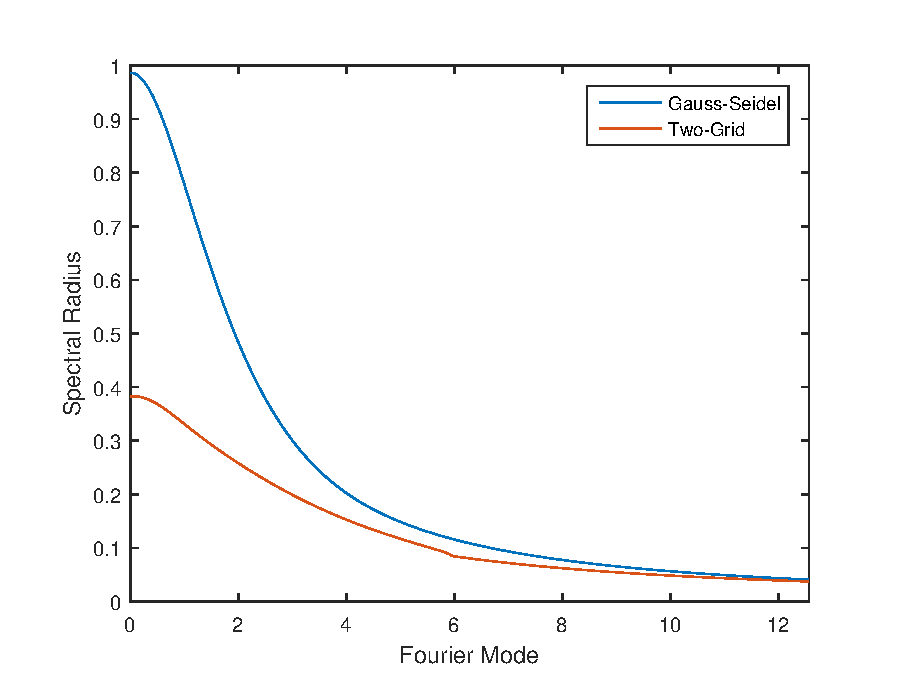
\includegraphics[width=0.485\textwidth]{images/P0_Fourier_69G.eps} \hfill
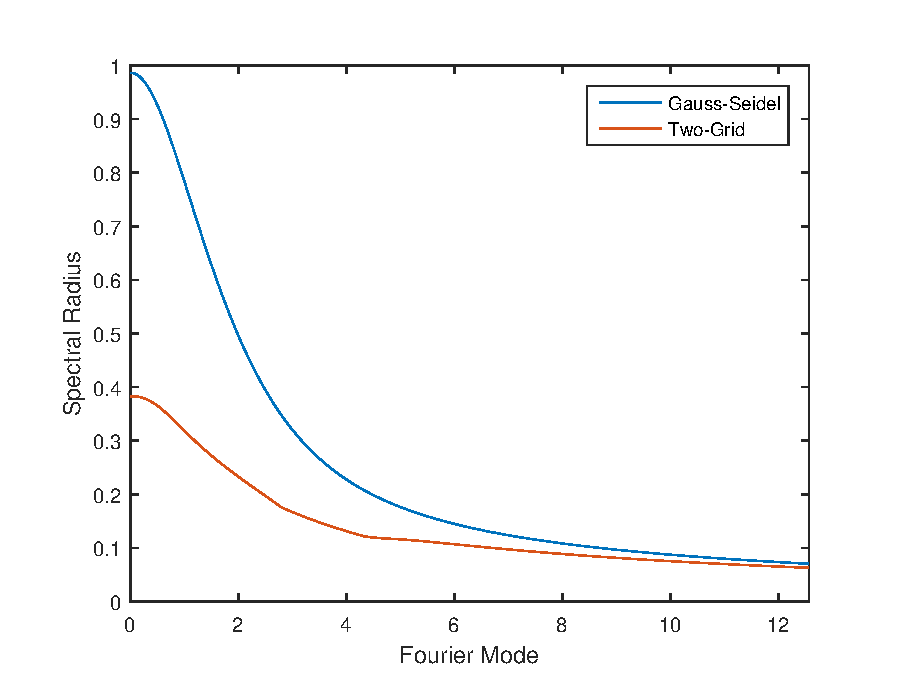
\includegraphics[width=0.485\textwidth]{images/P1_Fourier_69G.eps}
}
\end{frame}
%---------------------------
%%%%%%%%%%%%%%%%%%%%%%%%%%%%%%%%%%%%%%%%%%%%%%%%%%%%%%%%%%%%%%%%%%%%%%%%%%%%%%%%%%%%%%%%%%%%%%
%
\subsection{PDT results}
%---------------------------
\begin{frame}[t]\frametitle{Two-grid acceleration implementation in PDT}
\begin{block}{}
\begin{itemize}
	\item Successfully implemented and debugged
	\begin{itemize}
		\item Includes non-orthogonal  mesh configurations
		\item Includes multi-material configurations
	\end{itemize}
	\item Have tested the two-grid methodology on a homogeneous graphite block as well as a block with an air duct
	\item Iteration counts for a very large configuration (very optically thick) are similar to simple infinite medium calculations
\end{itemize}
\end{block}
\centering

Example: $S_8$ level-symmetric quadratures, 64,000 spatial DOFs, 99 energy groups (IM1 XS-data), run locally on 8 procs.
%\vspace{1mm}
\begin{table}
\footnotesize
\begin{tabular}{|c|c|c|}
\hline
Materials & Unaccelerated Iterations & Accelerated Iterations  \\
\hline \hline
Graphite Only & 2027 & 21 \\ \hline
Graphite + Air Duct & 2138 & 23 \\ \hline
\end{tabular}
\end{table}

%\vspace{2mm}
\begin{table}
\footnotesize
\begin{tabular}{|c|c|c|}
\hline
Materials & Unaccelerated Solve Time  & Accelerated Solve Time  \\
\hline \hline
Graphite Only & 51.67 hours & 31.23 minutes \\ \hline
Graphite + Air Duct & 54.5 hours & 35.56 minutes \\ \hline
\end{tabular}
\end{table}


\end{frame}
%---------------------------
%%%%%%%%%%%%%%%%%%%%%%%%%%%%%%%%%%%%%%%%%%%%%%%%%%%%%%%%%%%%%%%%%%%%%%%%%%%%%%%%%%%%%%%%%%%%%
\typeout{***********************************************************************************}
\typeout{Summary}

\section{Summary}
\subsection{}
%---------------------------

\begin{frame}[t]\frametitle{Work Summary and Status}

\begin{block}{DFEM Diffusion as an accelerator}
\begin{itemize}
\item Successfully developed and implemented an Modified Interior Penalty DFEM method as a diffusion synthetic accelerator for both \begin{enumerate}
\item within group iterations and 
\item thermal upscattering iterations
\end{enumerate}
\item MIP-DSA leads to symmetric positive definite matrices (PCG with AMG through HYPRE)
\item Excellent initial scaling results with PDT up to 132,000 cores.
\end{itemize}
\end{block}

\begin{block}{Next steps}
\begin{itemize}
\item Push into PDT's trunk repository
\item Further scaling tests
\item Apply to IM-1 experiments
\end{itemize}
\end{block}

\end{frame}
%---------------------------
%%%%%%%%%%%%%%%%%%%%%%%%%%%%%%%%%%%%%%%%%%%%%%%%%%%%%%%%%%%%%%%%%%%%%%%%%%%%%%%%%%%%%%%%%%%%%
\typeout{***********************************************************************************}
\typeout{We have reached the end}

\begin{frame}[plain]
   \frametitle{Thank you}

\vspace{25mm}

\begin{columns}[b]

\column{0.7\textwidth}

\centering

{\Large Questions?}


\end{columns}

\vspace{10mm}

\begin{columns}[b]

\column{0.5\textwidth}
\centering
{}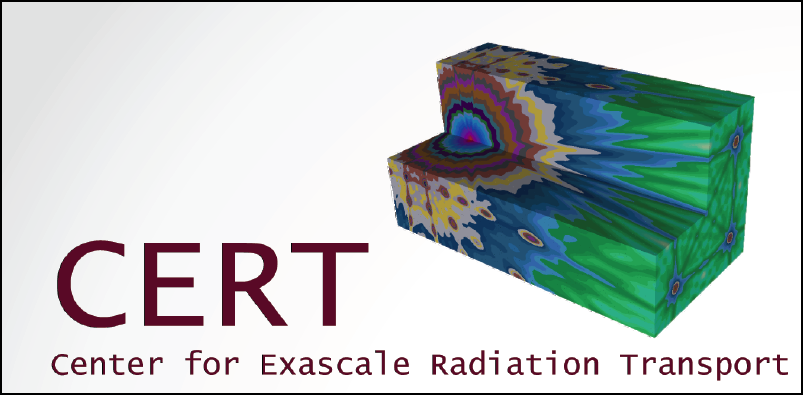
\includegraphics[width=0.75\figwidth]{images/CERT_logo.png}\\

\column{0.5\textwidth}
\centering
{}
\includegraphics[width=0.70\figwidth]{images/tamu_engineering.png}\\

\end{columns}

\end{frame}
%%%%%%%%%%%%%%%%%%%%%%%%%%%%%%%%%%%%%%%%%%%%%%%%%%%%%%%%%%%%%%%%%%%%%%%%%%%%%%%%%%%%%%%%%%%%%

%---------------------------
\setbeamerfont{frametitle}{size=\small}
\begin{frame}[t]\frametitle{2D Exactly-Linear Transport Solutions - mean value coordinates}
\begin{block}{}
\begin{equation*}
\begin{aligned}
\mu \frac{\partial  \psi}{\partial x} + \eta \frac{\partial  \psi}{\partial y} + \sigma_t \psi &= Q(x,y,\mu,\eta) \\
\psi (x,y,\mu,\eta) = a x + b y + c \mu + d \eta + e& , \qquad  \phi (x,y) = 2 \pi \left(   a x + b y  + e  \right)
\end{aligned}
\end{equation*}
\end{block}
\centering
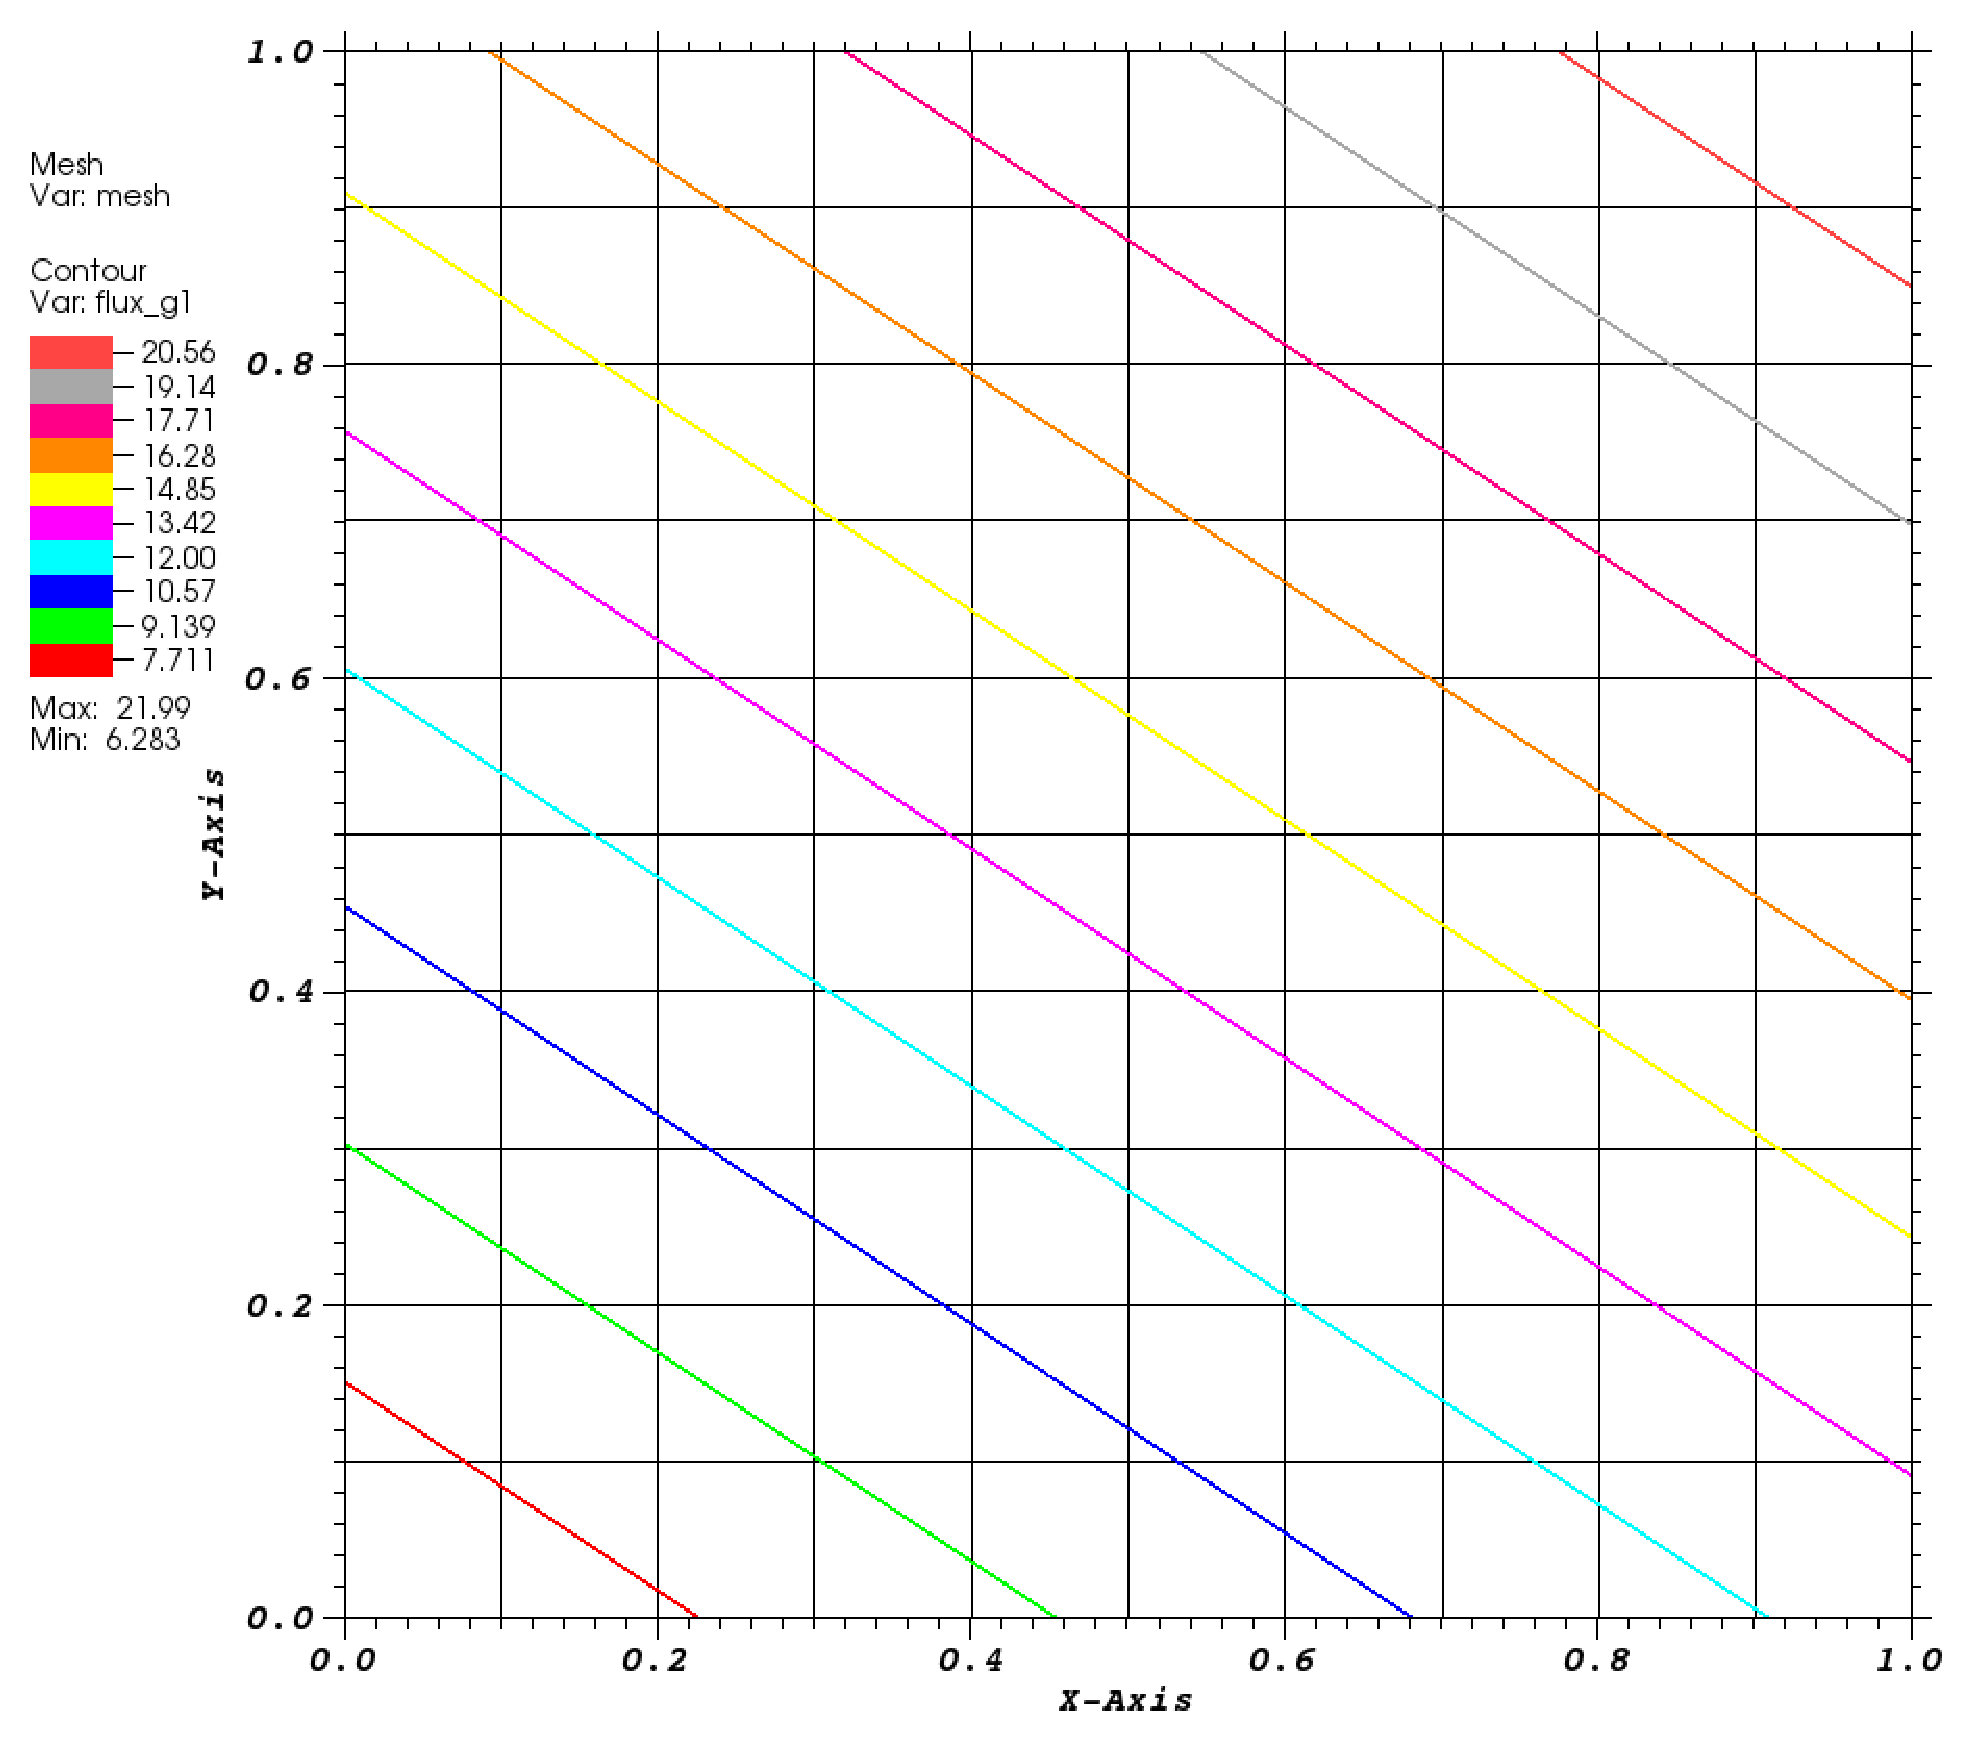
\includegraphics[width=0.25\textwidth]{images/cart_MV_k1.eps} 
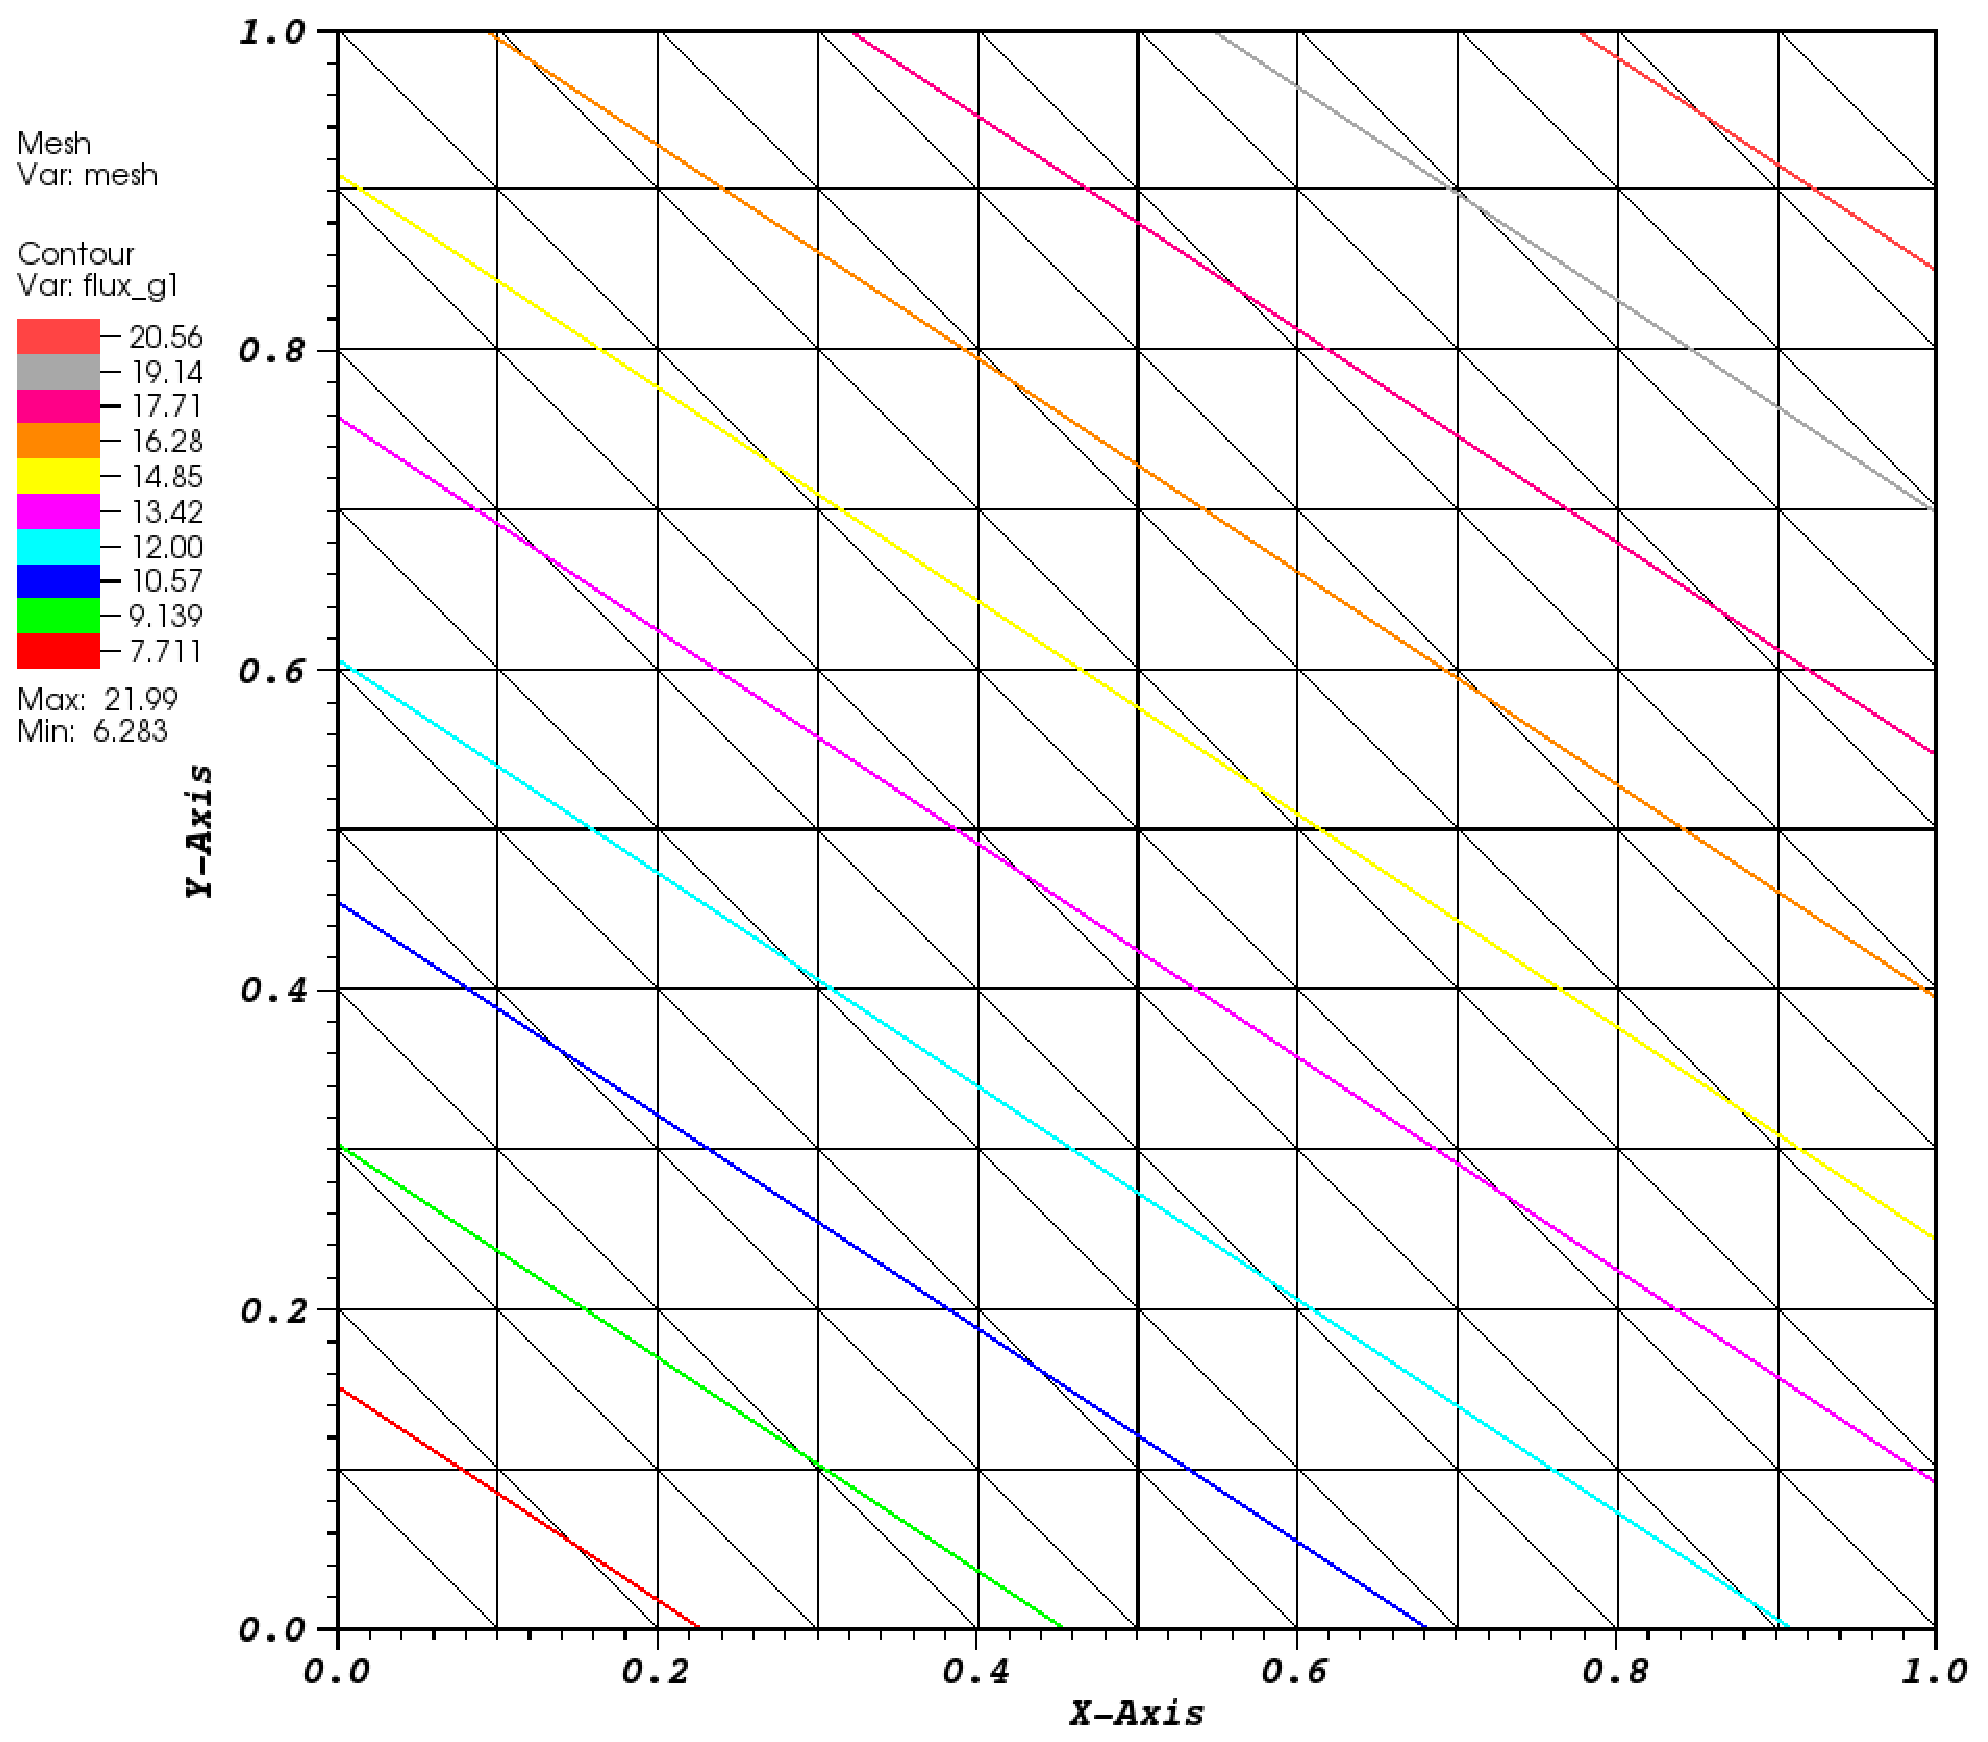
\includegraphics[width=0.25\textwidth]{images/tri_MV_k1.eps} 
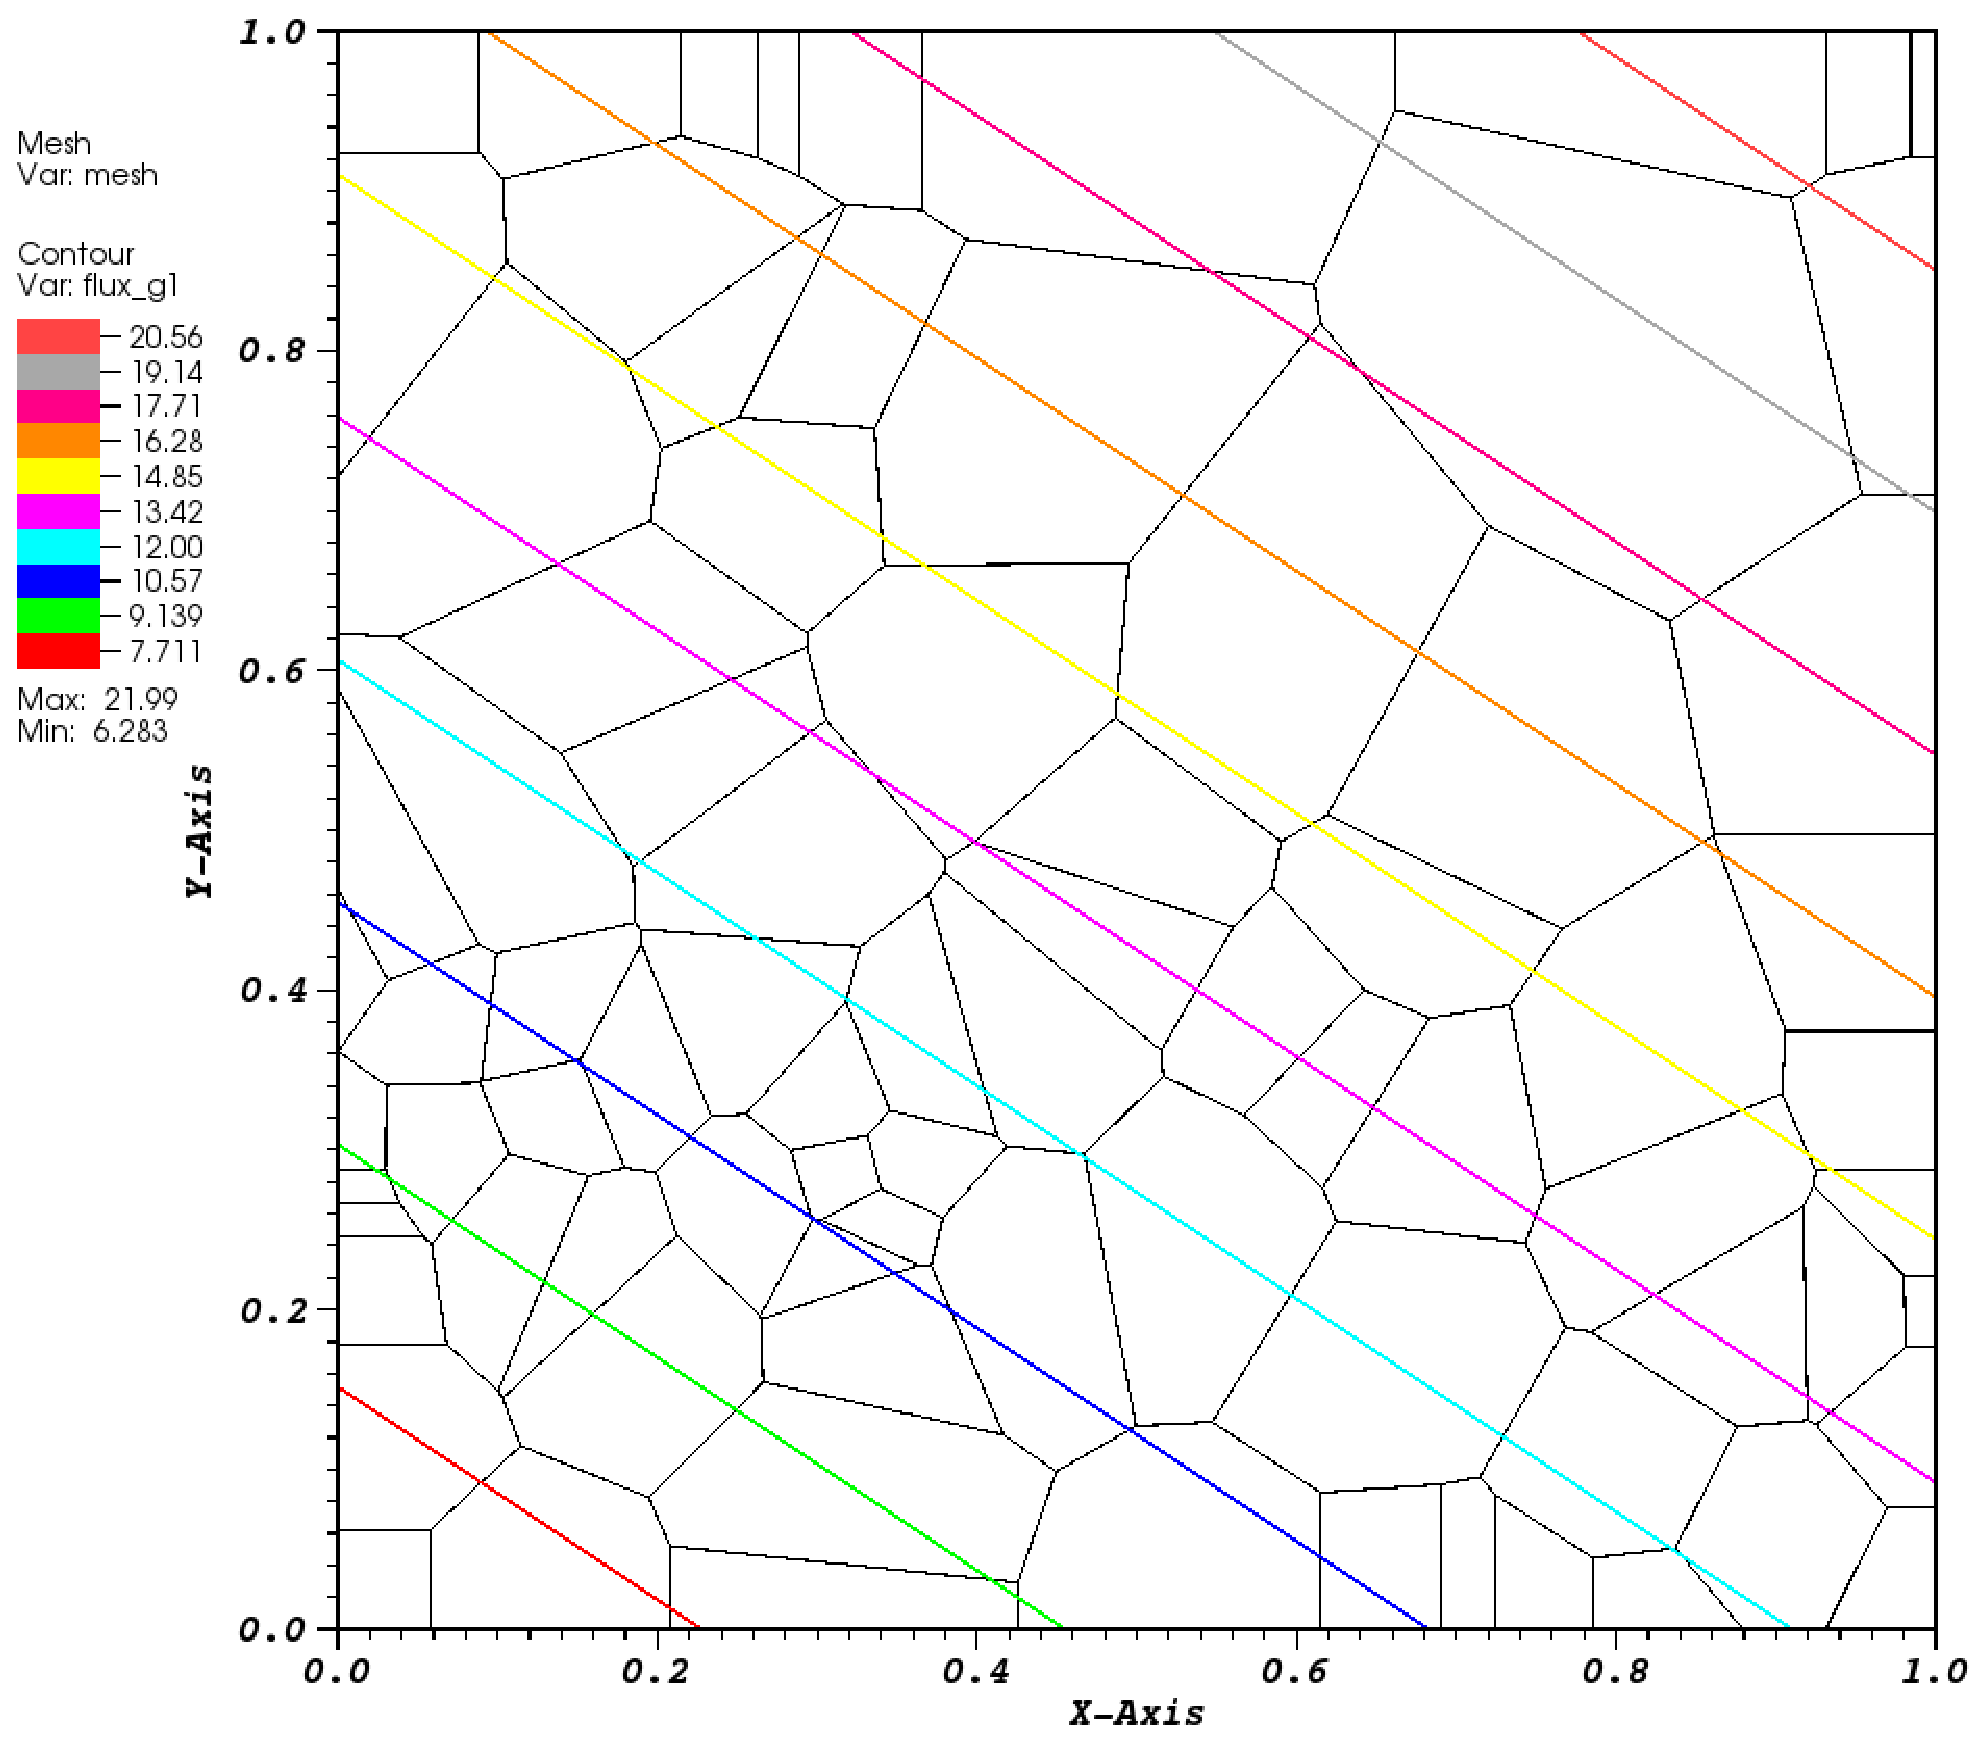
\includegraphics[width=0.25\textwidth]{images/shes_poly_MV_k1.eps} 
\vspace{0.2cm}
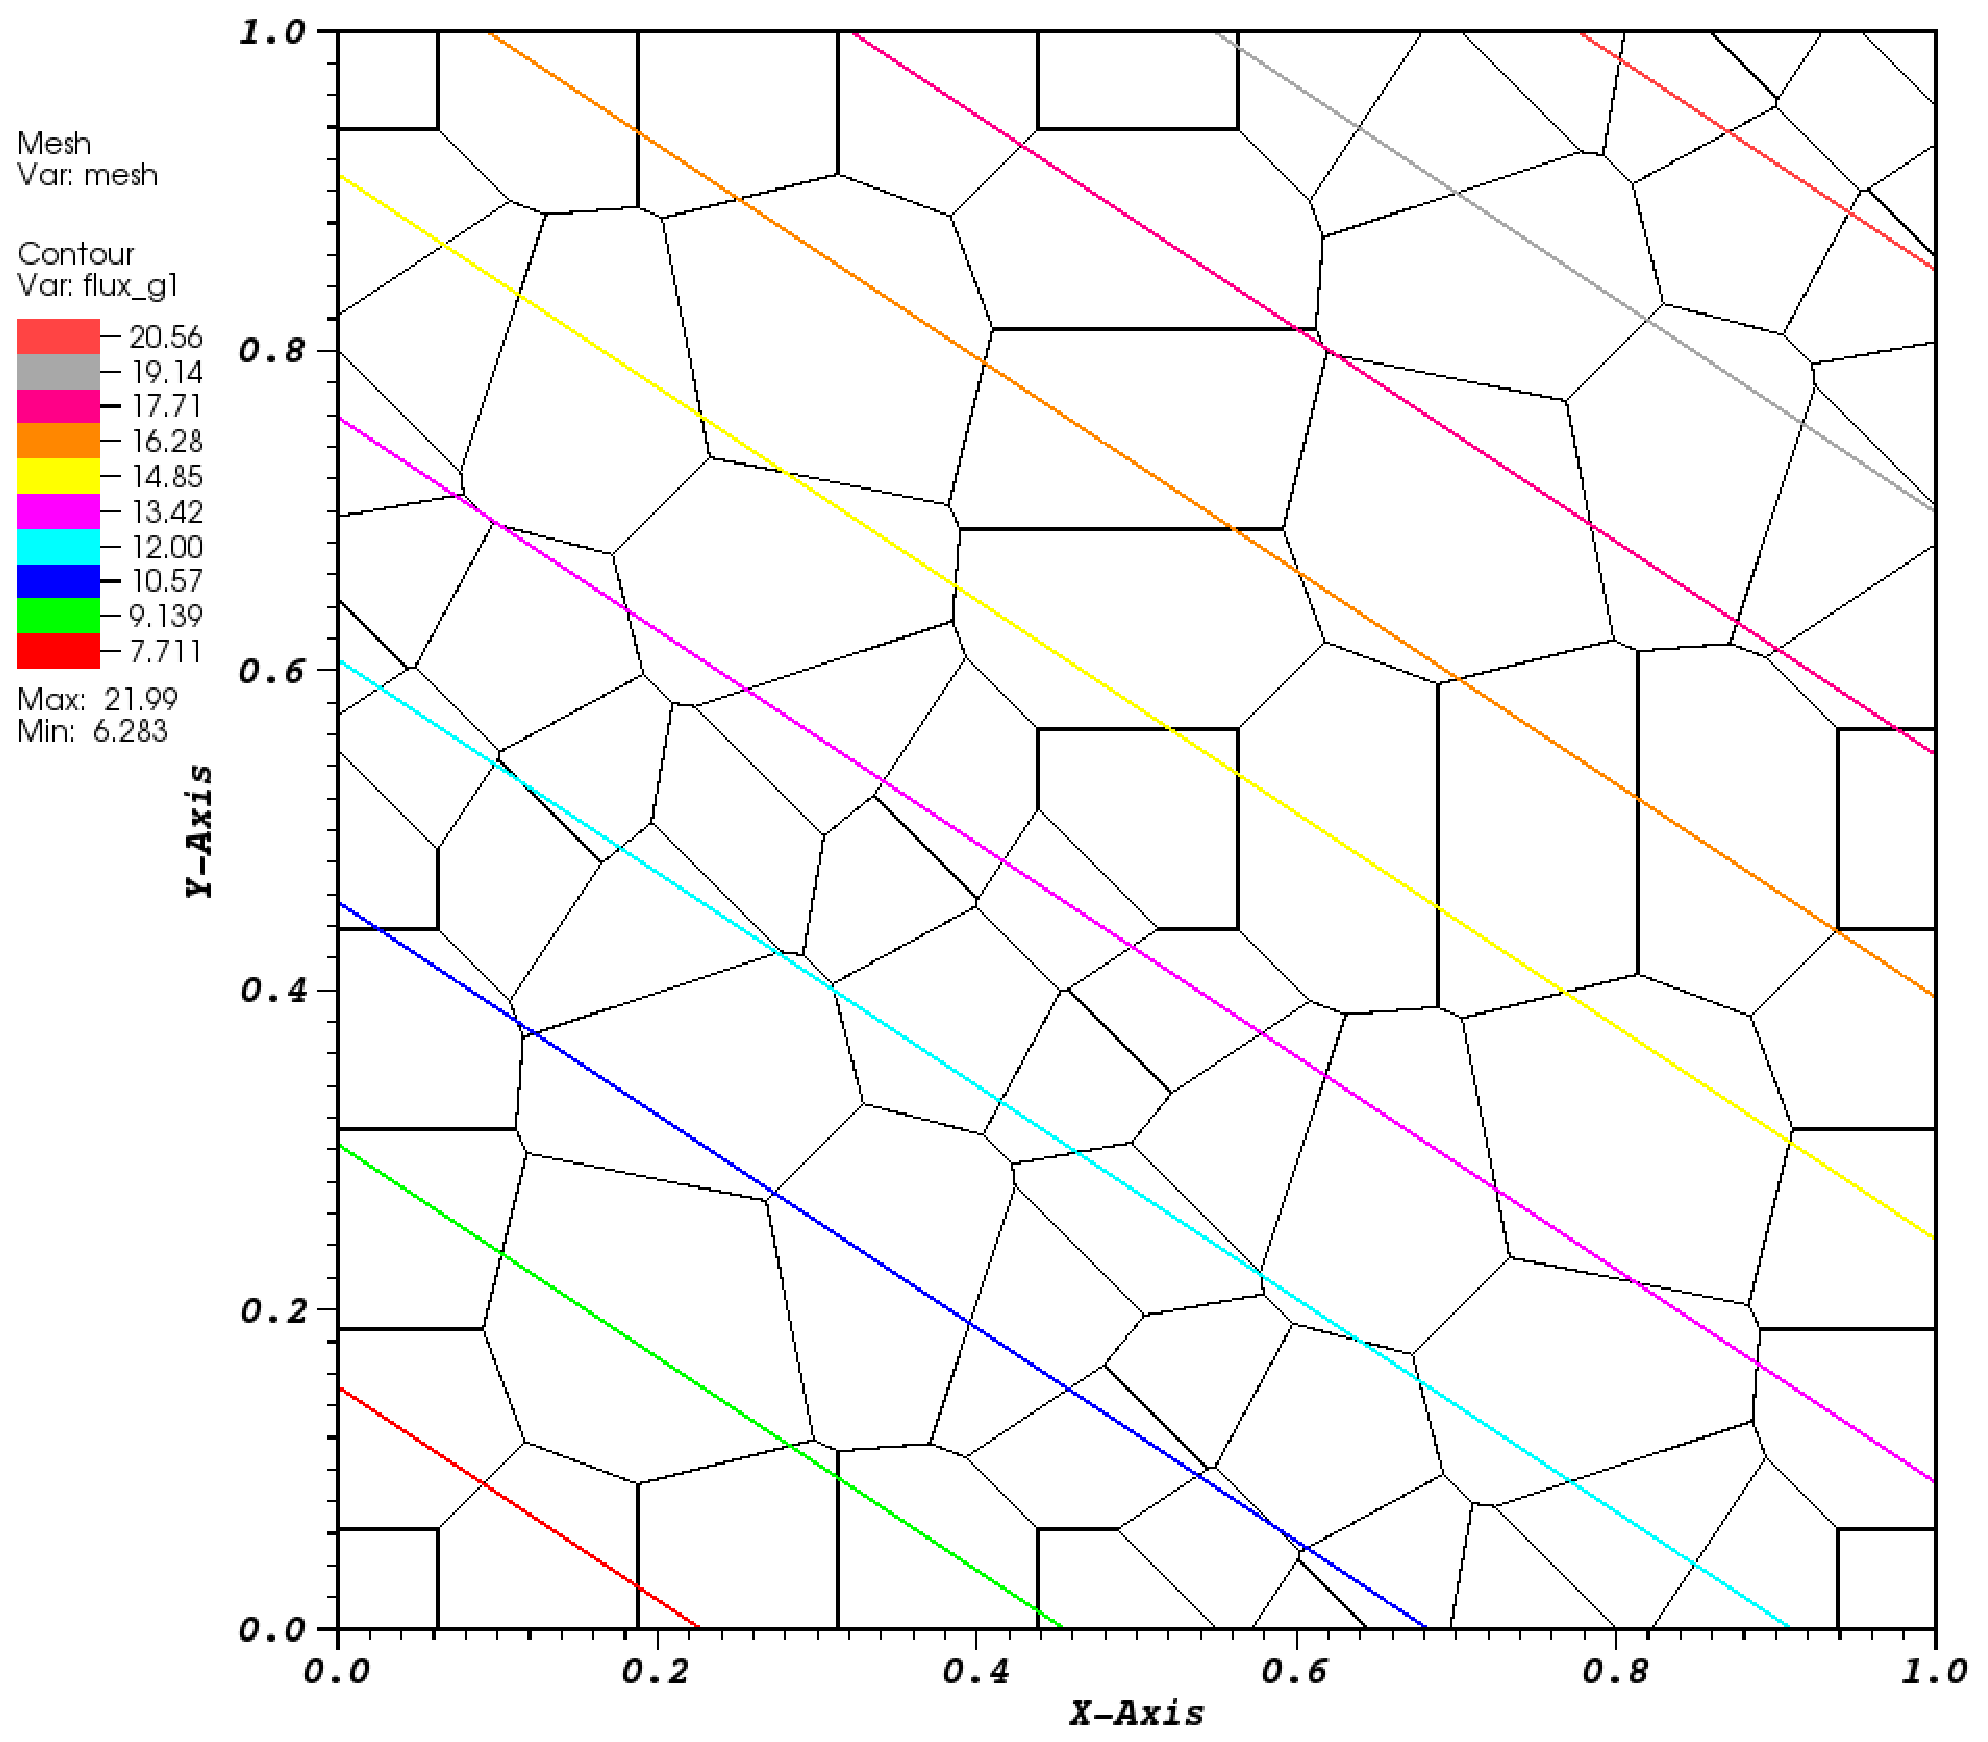
\includegraphics[width=0.25\textwidth]{images/smooth_poly_MV_k1.eps} 
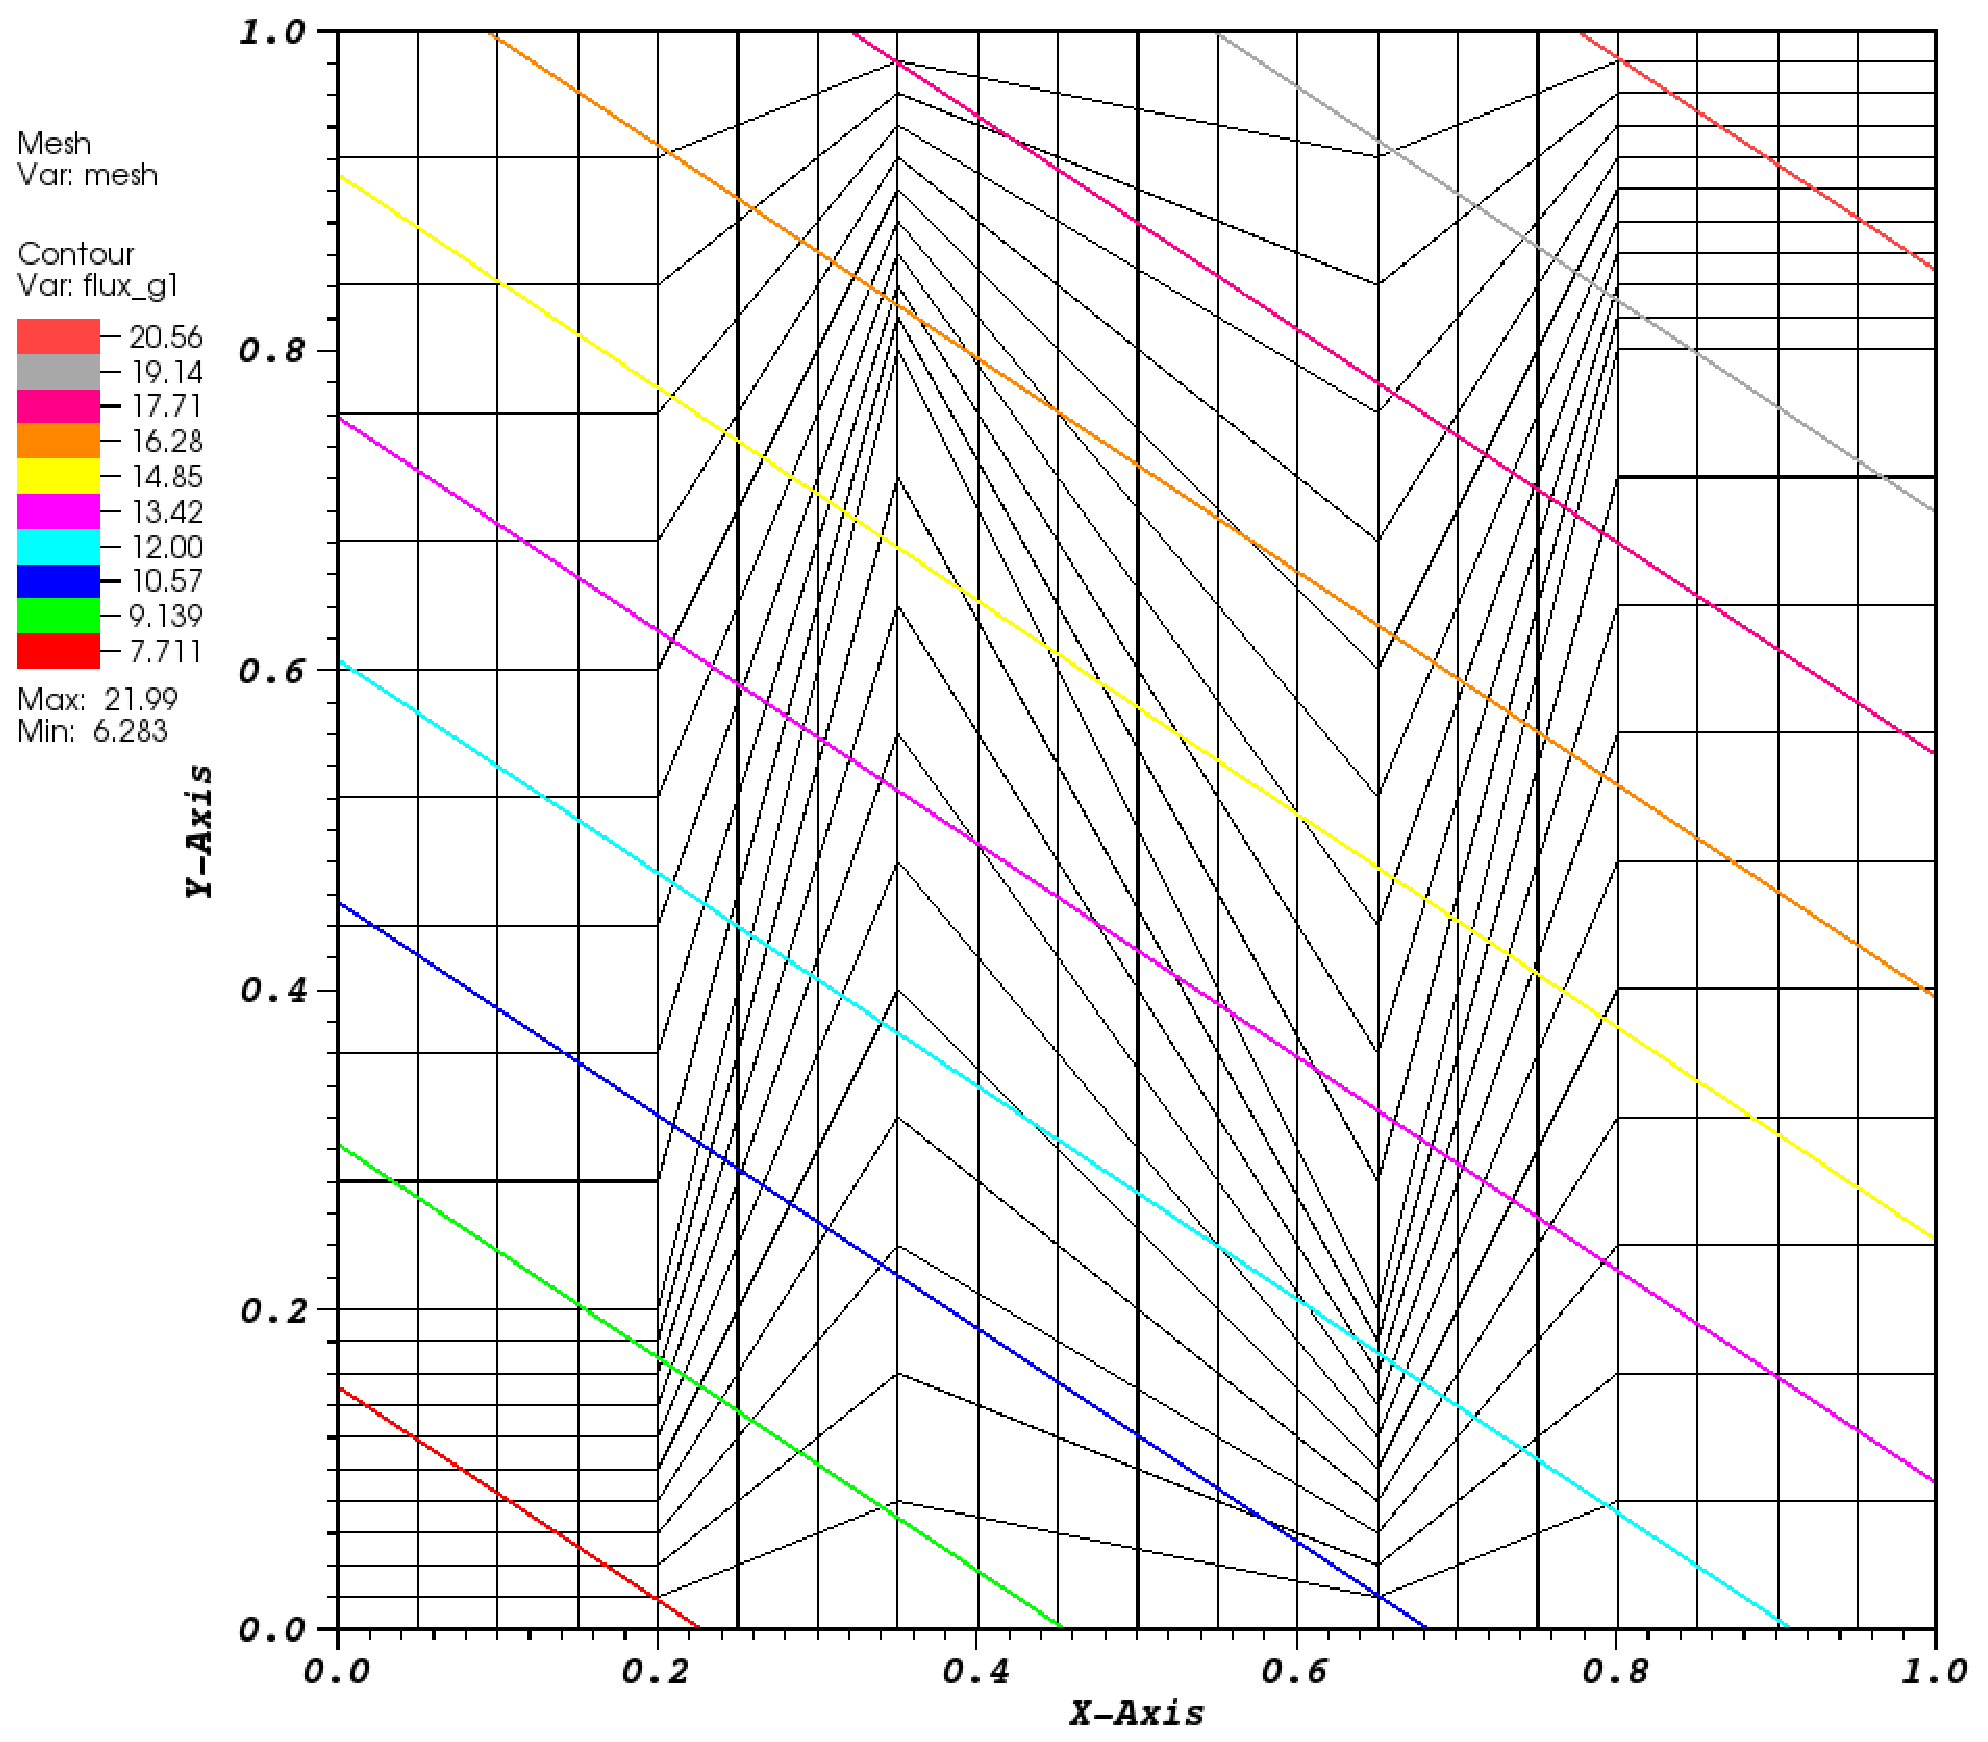
\includegraphics[width=0.25\textwidth]{images/z_quad_MV_k1.eps}
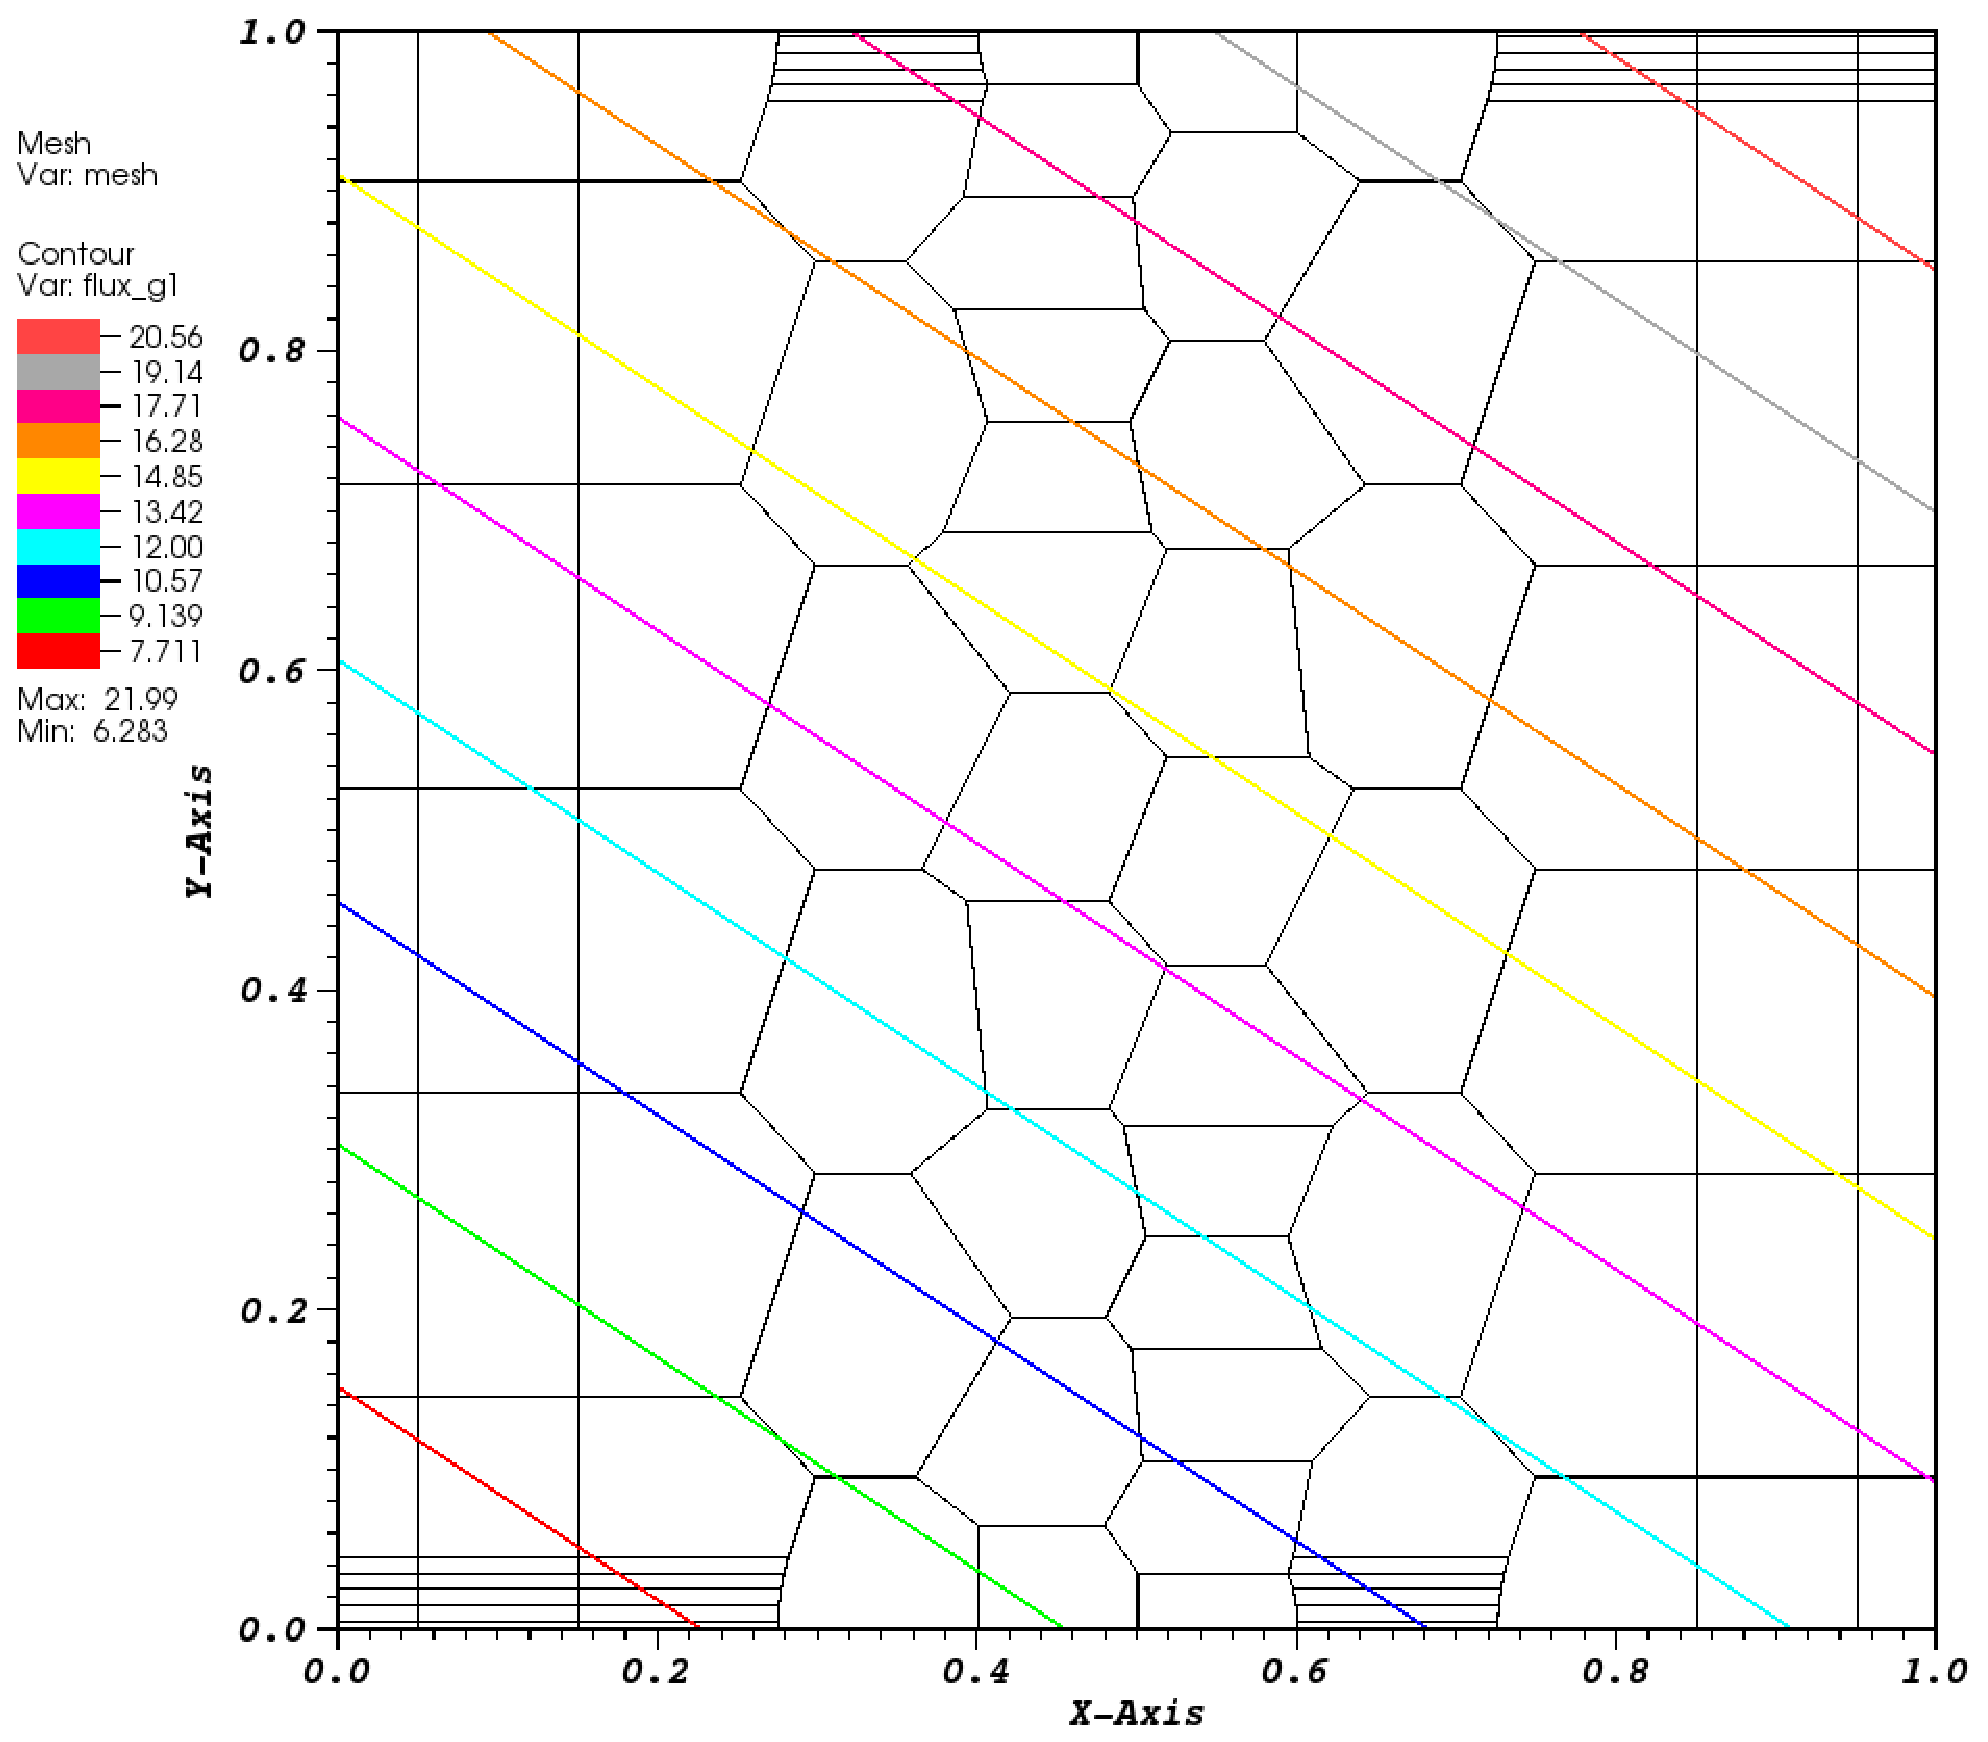
\includegraphics[width=0.25\textwidth]{images/z_poly_MV_k1.eps}
\end{frame}
%---------------------------
\setbeamerfont{frametitle}{size=\small}
\begin{frame}[t]\frametitle{SIP exactly linear solutions on 3D polyhedral meshes using the PWL basis functions}
\centering
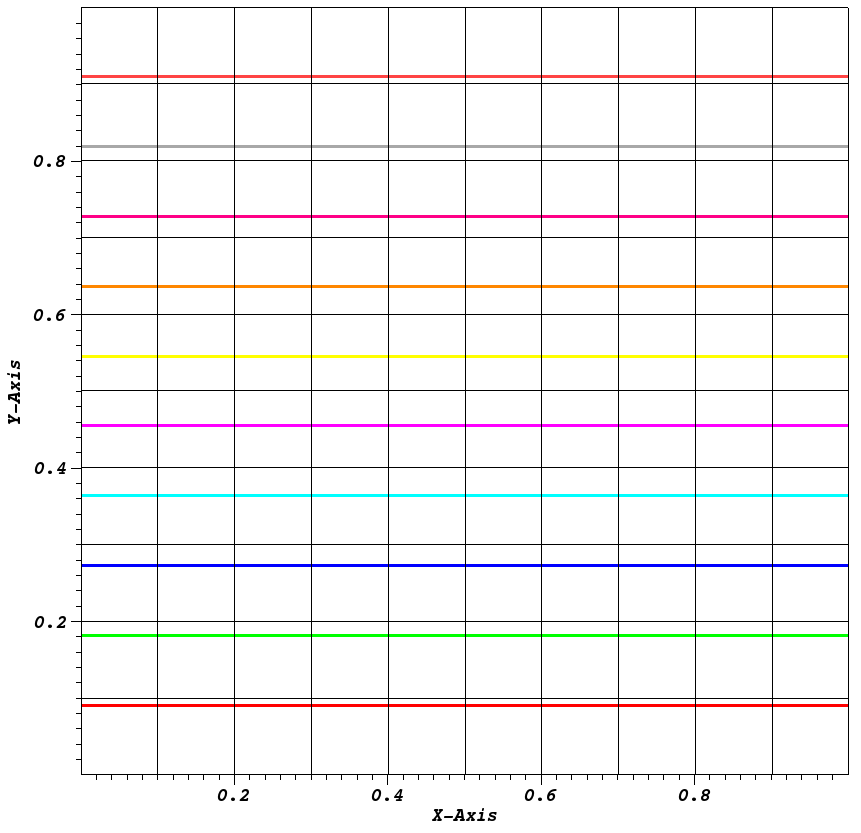
\includegraphics[width=0.32\textwidth]{images/cart_lin_contour.png} 
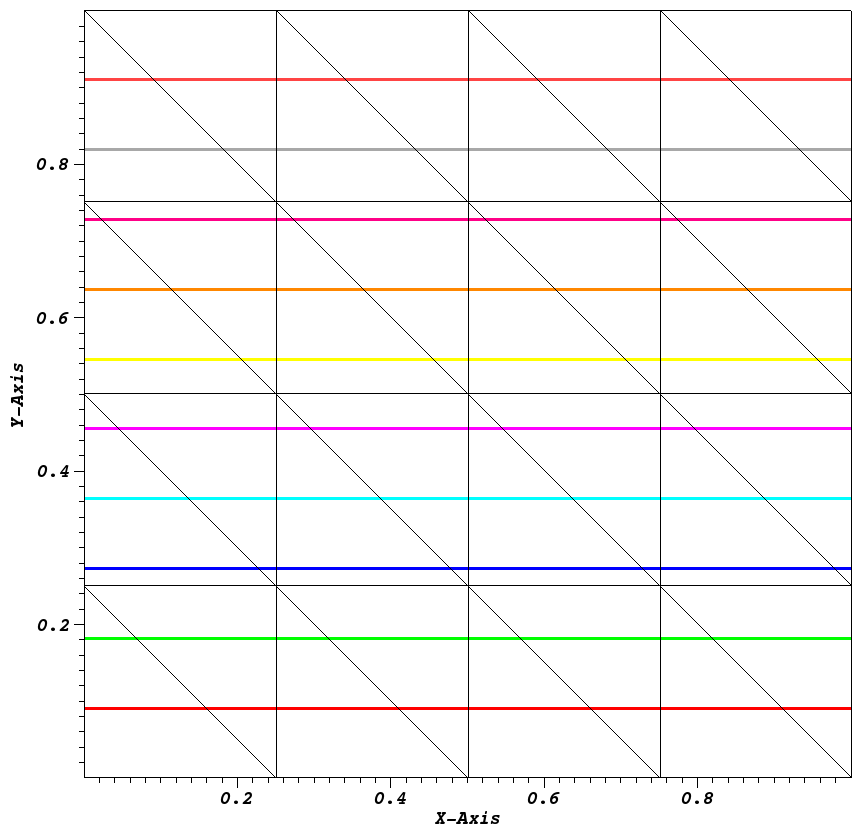
\includegraphics[width=0.32\textwidth]{images/tri_lin_contour.png} \\
\vspace{0.2cm}
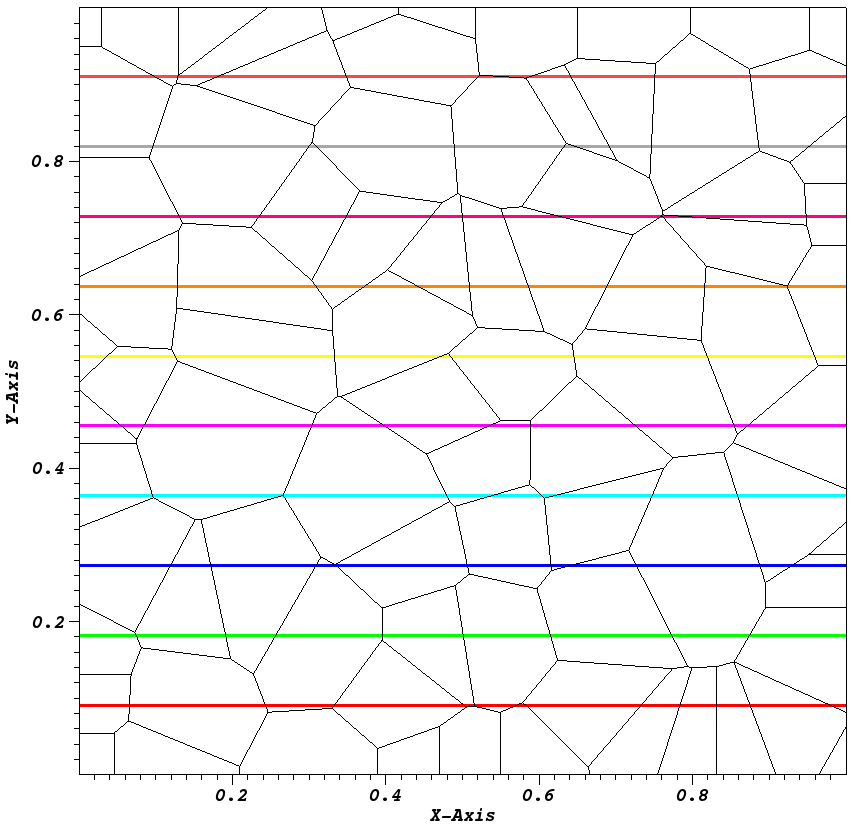
\includegraphics[width=0.32\textwidth]{images/poly_lin_contour.png} 
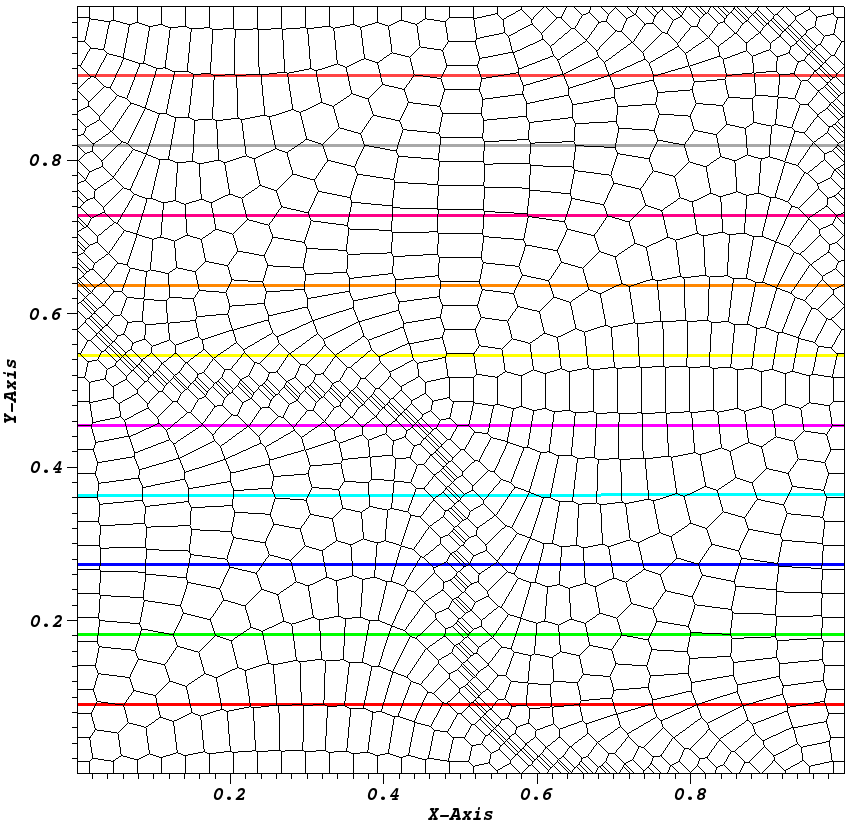
\includegraphics[width=0.32\textwidth]{images/sine_poly_lin_contour.png} 
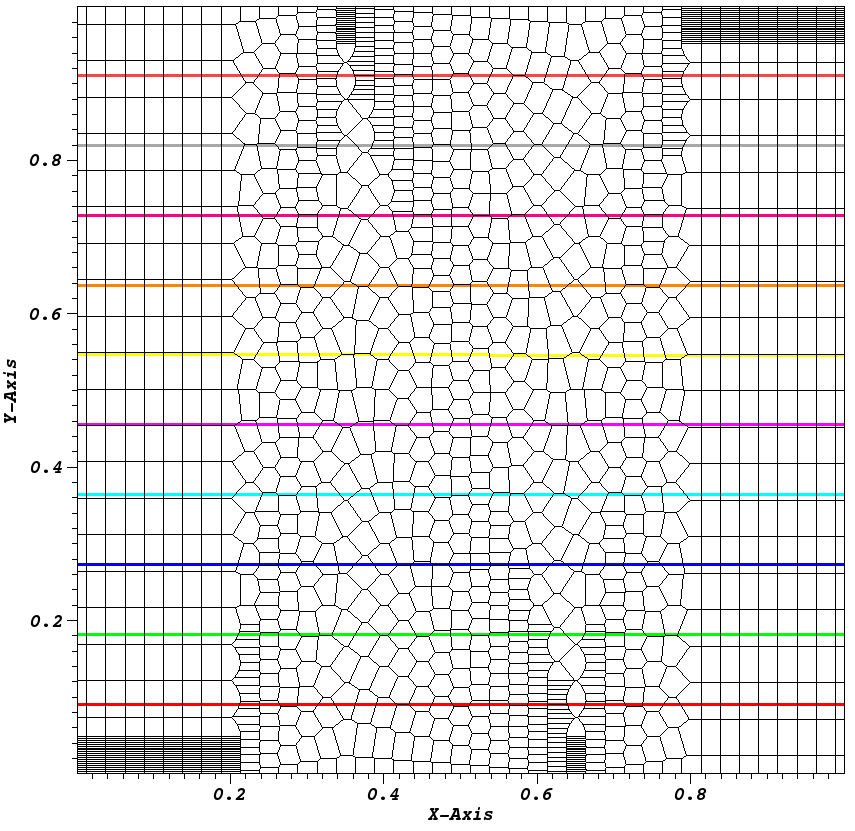
\includegraphics[width=0.32\textwidth]{images/z_poly_lin_contour.png} 
\end{frame}
%---------------------------
% QUAD MMS SOLUTION - CURRENTLY COMMENTED OUT
\iffalse
\setbeamerfont{frametitle}{size=\small}
\begin{frame}[t]\frametitle{SIP convergence study - quadratic solution on 3D cube using the PWL basis functions}
\begin{block}{}
	\begin{equation*}
		\begin{aligned}
		\Phi(x,y,z) =& x y z (L_x - x)  (L_y - y)  (L_z - z) \\
		L_x& = L_x = L_x = 1.0
		\end{aligned}
	\end{equation*}
\end{block}
\centering
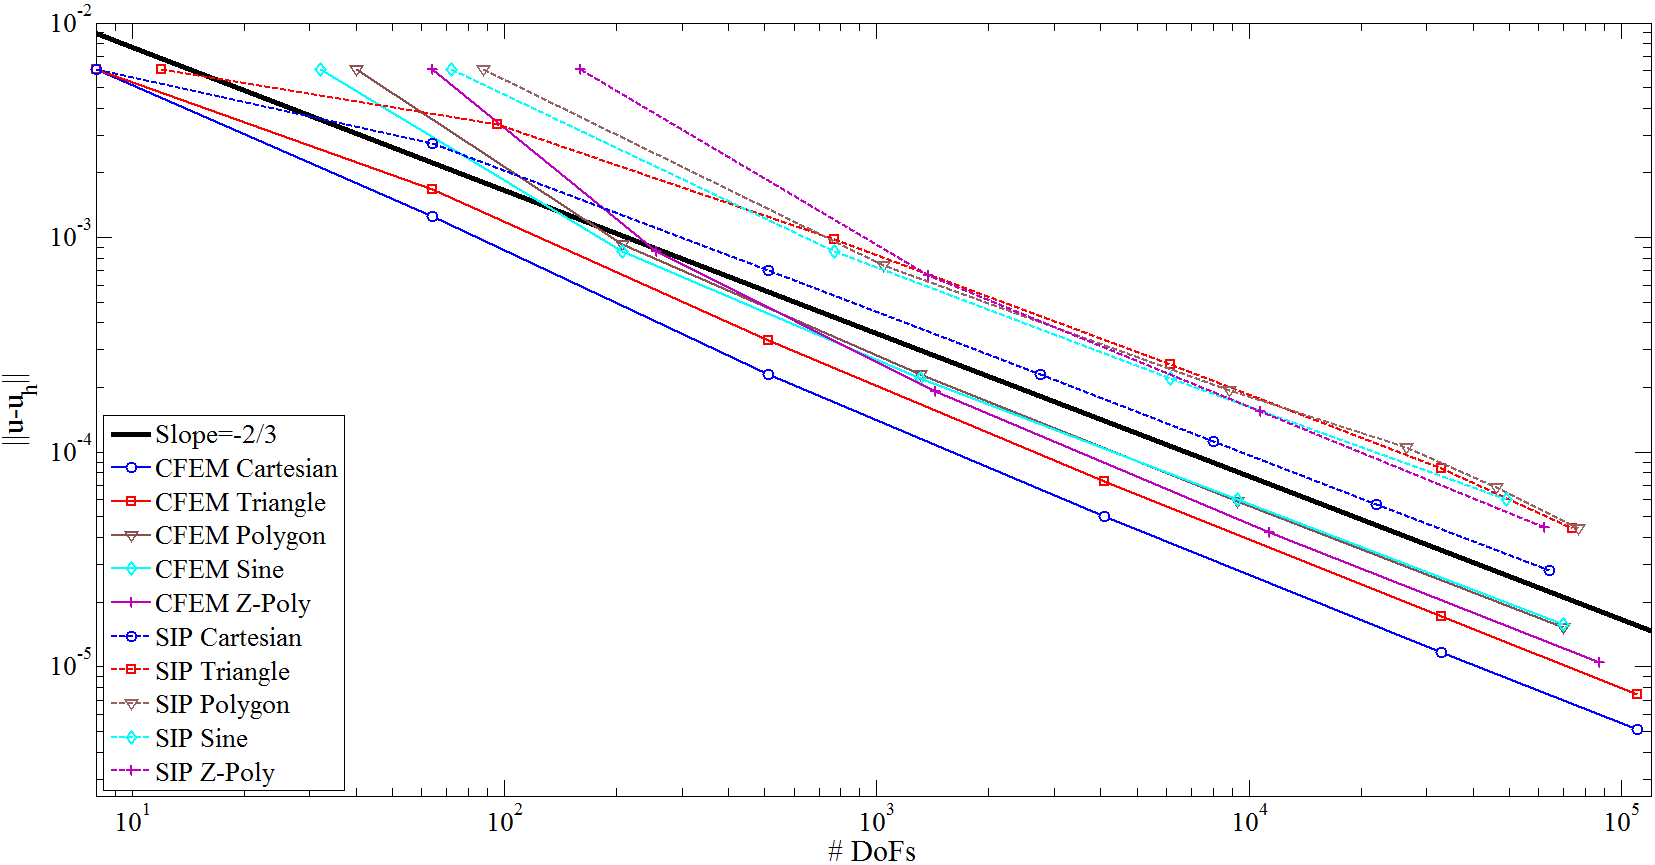
\includegraphics[width=0.9\textwidth]{images/sip_quad_full_paint.png} 
\end{frame}
\fi
%---------------------------
\setbeamerfont{frametitle}{size=\small}
\begin{frame}[t]\frametitle{SIP convergence study - gaussian solution on 3D cube using the PWL basis functions}
\begin{block}{}
	\begin{equation*}
		\begin{aligned}
		\Phi(x,y,z) = x y z (L_x - x)  (L_y - y)  (L_z - z) \exp(-({\bf r} - {\bf r}_0) \cdot ({\bf r} - {\bf r}_0))\\
		L_x = L_x = L_x = 1.0 , \qquad {\bf r}_0 = (3/4,3/4,3/4)
		\end{aligned}
	\end{equation*}
\end{block}
\centering
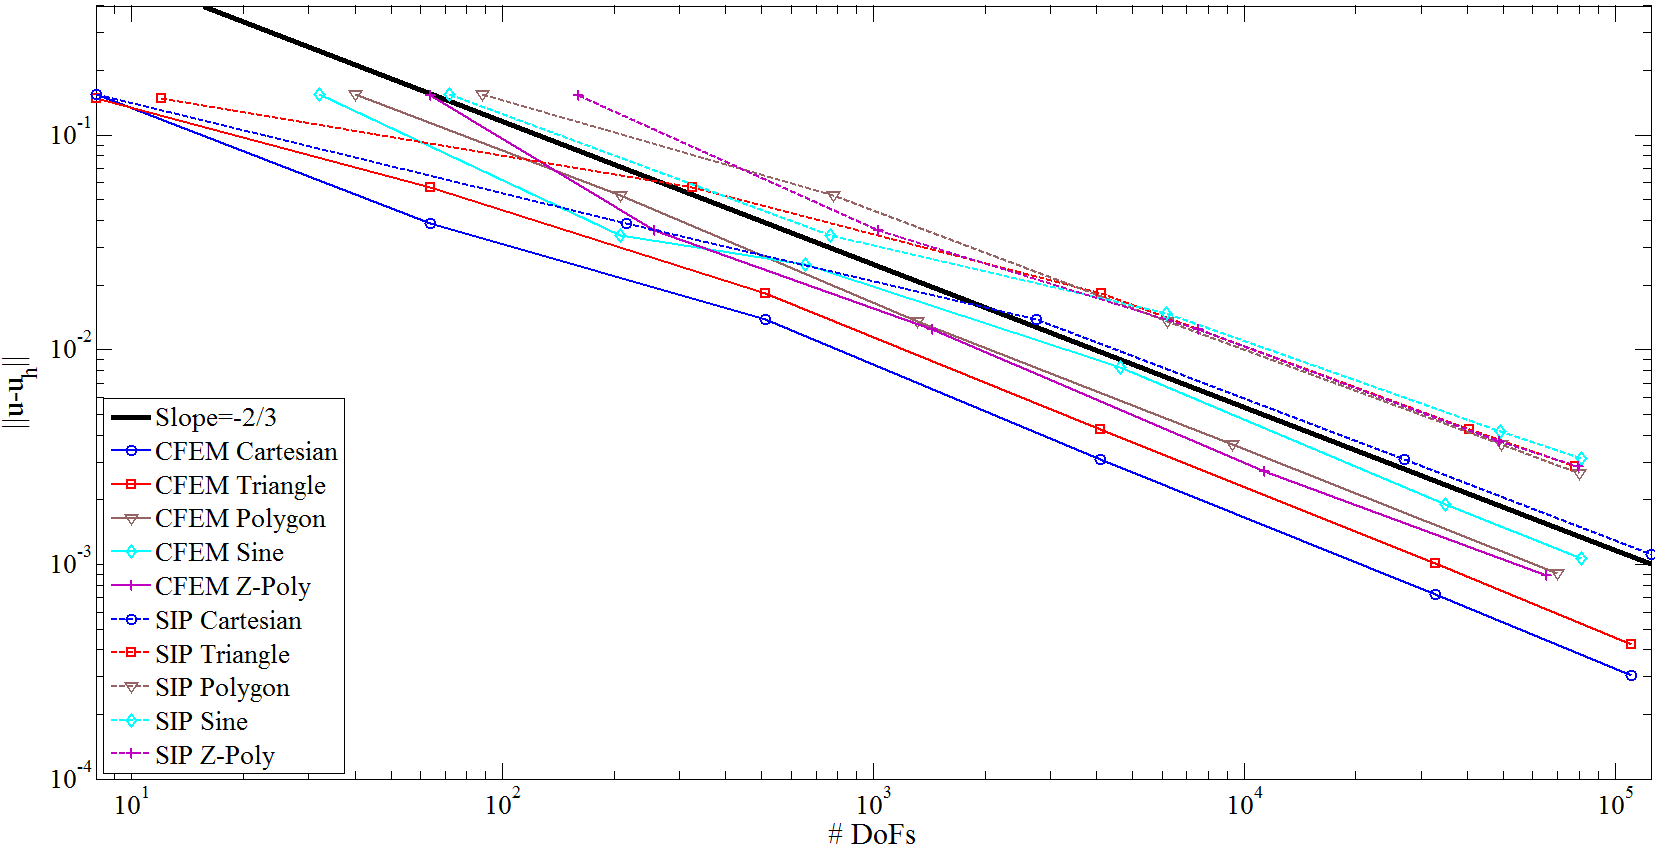
\includegraphics[width=0.9\textwidth]{images/sip_gauss_full_paint.png} 
\end{frame}
%---------------------------

%%%%%%%%%%%%%%%%%%%%%%%%%%%%%%%%%%%%%%%%%%%%%%%%%%%%%%%%%%%%%%%%%%%%%%%%%%%%%%%%%%%%%%%%%%%%%

\end{document}

